%!TEX root = ../thesis.tex

\chapter{Adaptivity}
\label{adp_sec:main}
\section{Introduction}
\paragraph{}
The main objective of this chapter is to introduce a way that can improve the overall mesh quality by refinement automatically and adaptively.
Unnecessary refinement in the region which contributes little to the improvement to the accuracy will be largely prevented.
The expressions related to the eigenvalues of the SBFEM formulation representing the quantity of the error in the interpolation are adopted as one of the error indicators, together with the area and other geometric properties of the Scaled Boundary Finite Element.
A machine learning model using the Multilayer Perceptron (MLP) is trained to determine whether a Scaled Boundary Finite Element needs refinement or not based on all these information.

\paragraph{}
The proposed method enhances the SBFEM with quad-tree mesh introduced in Sec.~\ref{qdt_sec:main} and the outstanding features of the method are:
\begin{itemize}
    \item No human effort involvement in mesh refinement
    \item Smart refinement detection
    \item Flexible refinement criteria
\end{itemize}

\paragraph{}
This chapter is organized as follows.
The error indicators used in the proposed method will be introduced first.
After that, a machine learning algorithm that can be trained to determine the necessity of the refinement of a cell based on these indicators.
Furthermore, a triangle merging algorithm is developed to bypass the lack of some error indicators in first order triangle element.
Finally, the matrix representation of NURBS curves is introduced to improve the computational efficiency and the robustness of the NURBS related calculation.
The accuracy and the convergence properties of the proposed techniques are demonstrated with benchmark problems in the context of linear elasticity, followed by concluding remarks in the last section.


\section{Error indicator}
\label{adap_sec:error_indicator}

\subsection{Mesh Size}
\paragraph{}
The area of a subdomain will apparently influence the accuracy of the result.
Generally speaking, a larger subdomain tends to have a higher error.
The area of any polygon in fig.~\ref{adap_ei_polygon} can be calculated as 

\begin{equation}
    S = \frac{1}{2}
        \sum_{k=1}
        \left(
            x_k y_{k+1} - x_{k+1} y_k
        \right)
\end{equation}

\begin{figure}[!ht]
    \centering
    \scalebox{1}{
        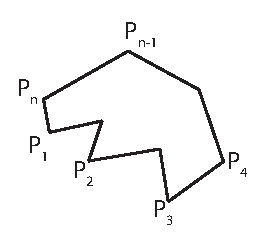
\includegraphics{adaptivity/images/adap_ei_polygon.eps}
    }
    \caption{A polygon with $n$ vertexes}
    \label{adap_ei_polygon}
\end{figure}

%   ----    %
\subsection{Mesh Quality}
\paragraph{}
Mesh quality is another important factor that influence the accuracy.
In SBFEM, mesh quality is highly related to the minimal angle formed by the intersecting lines connected by scaling center and adjacent polygon vertexes.
An extremely smaller angel may raise numerical stability issue and hence decrease the accuracy of the result.


%   ----    %

\subsection{Eigenvalue in SBFEM}
\paragraph{}
The displacement solution in SBFEM can be calculated as
\begin{equation}
    u(\xi)
\end{equation}




\section{Machine learning}
\paragraph{}
Due to the fact that there are a few error indicators, it could be hard to determine the relationship between them and whether a subdomain needs refinement or not.
As a result, specific technique is required in order to search for the patterns in the data to find this relationship.
After that, the final decision which is a binary classification in this case as each subdomain will be labeled as ``refine'' or ``not refine'' can be made based on the input of the error indicators explained in Sec.~\ref{adap_sec:error_indicator}.
Hence, the discovery of regularities plays a key role in the adaptive analysis and an automatic discovery of regularities is usually associated with pattern recognition by the help of algorithms.

%   ----    %
\subsection{Training Set}
\paragraph{}
The training set is determined by numerical examples in Fig.~\ref{adap_fig:svm_train_chole} and Fig.~\ref{adap_fig:svm_train_cantilever}.
The training data is annotated with whether a subdomain is refined or not and the model can study the data and learn to classify each subdomain based on all four features explained in \ref{adap_sec:error_indicator}.
\begin{figure}[!ht]
    \centering
    \begin{subfigure}[b]{0.5\linewidth}
        \scalebox{0.5}{
            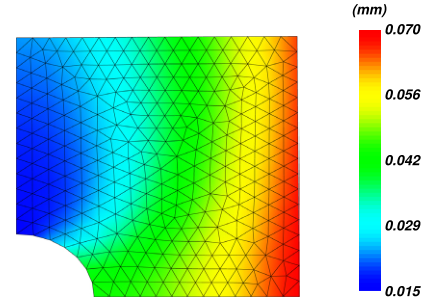
\includegraphics{adaptivity/images/adap_svm_train_chole_0.png}
        }
        \caption{Mesh and displacement field before refinement}
    \end{subfigure}
    \begin{subfigure}[b]{0.5\linewidth}
        \scalebox{0.45}{
            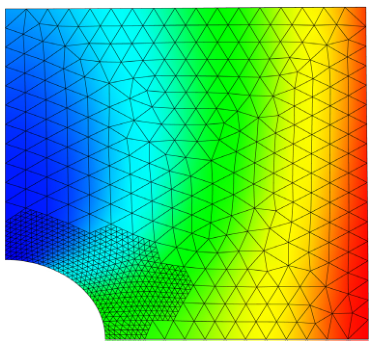
\includegraphics{adaptivity/images/adap_svm_train_chole_1.png}
        }
        \caption{Mesh and displacement field after refinement}
    \end{subfigure}
    \caption{Mesh refinement for square plate with circular hole \citep{Duval2018}}
    \label{adap_fig:svm_train_chole}
\end{figure}

\begin{figure}[!ht]
    \centering
    \begin{subfigure}[b]{0.4\linewidth}
        \scalebox{0.6}{
            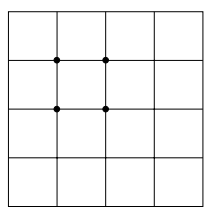
\includegraphics{adaptivity/images/adap_svm_train_cantilever_0.png}
        }
    \end{subfigure}
    \begin{subfigure}[b]{0.4\linewidth}
        \scalebox{0.6}{
            
\includegraphics{adaptivity/images/adap_svm_train_cantilever_1.png}
        }
    \end{subfigure}\\
    \begin{subfigure}[b]{1\linewidth}
        \centering
        \scalebox{0.7}{
            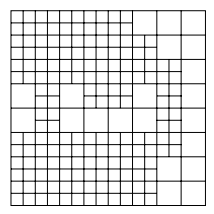
\includegraphics{adaptivity/images/adap_svm_train_cantilever_2.png}
        }
    \end{subfigure}
    \caption{Mesh refinement of a short cantilever beam \citep{Zienkiewicz2005500}}
    \label{adap_fig:svm_train_cantilever}    
\end{figure}
%
With the same examples, uniform mesh of quadtree is conducted and the same region are marked as refined as shown in Fig.~\ref{adap_fig:svm_train_my}.
\begin{figure}[!ht]
    \centering
    \begin{subfigure}[b]{1\linewidth}
        \centering
        \scalebox{0.25}{
            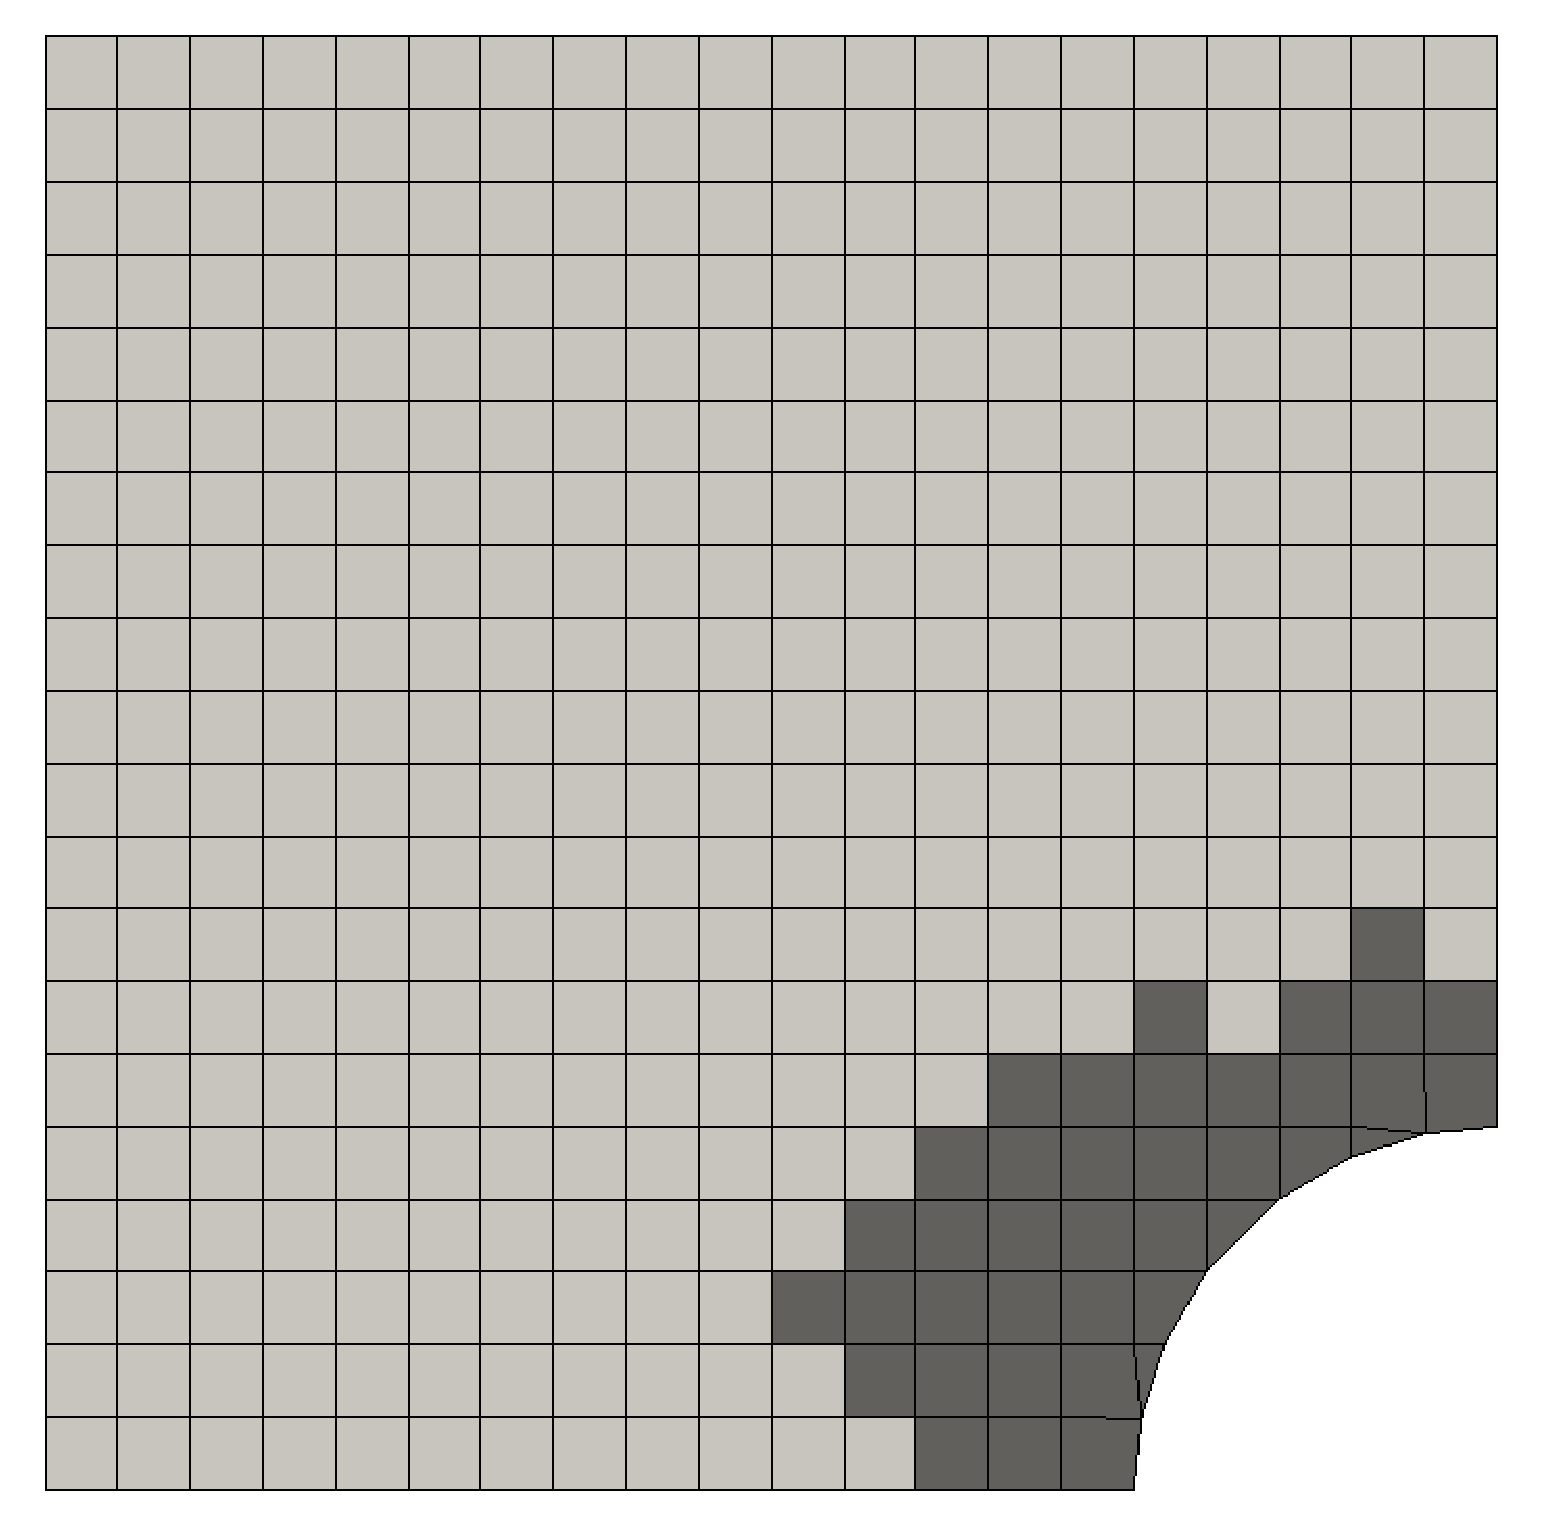
\includegraphics{adaptivity/images/adap_svm_train_my_chole.eps}
        }
    \end{subfigure}
    \begin{subfigure}[b]{0.49\linewidth}
        \scalebox{0.25}{
            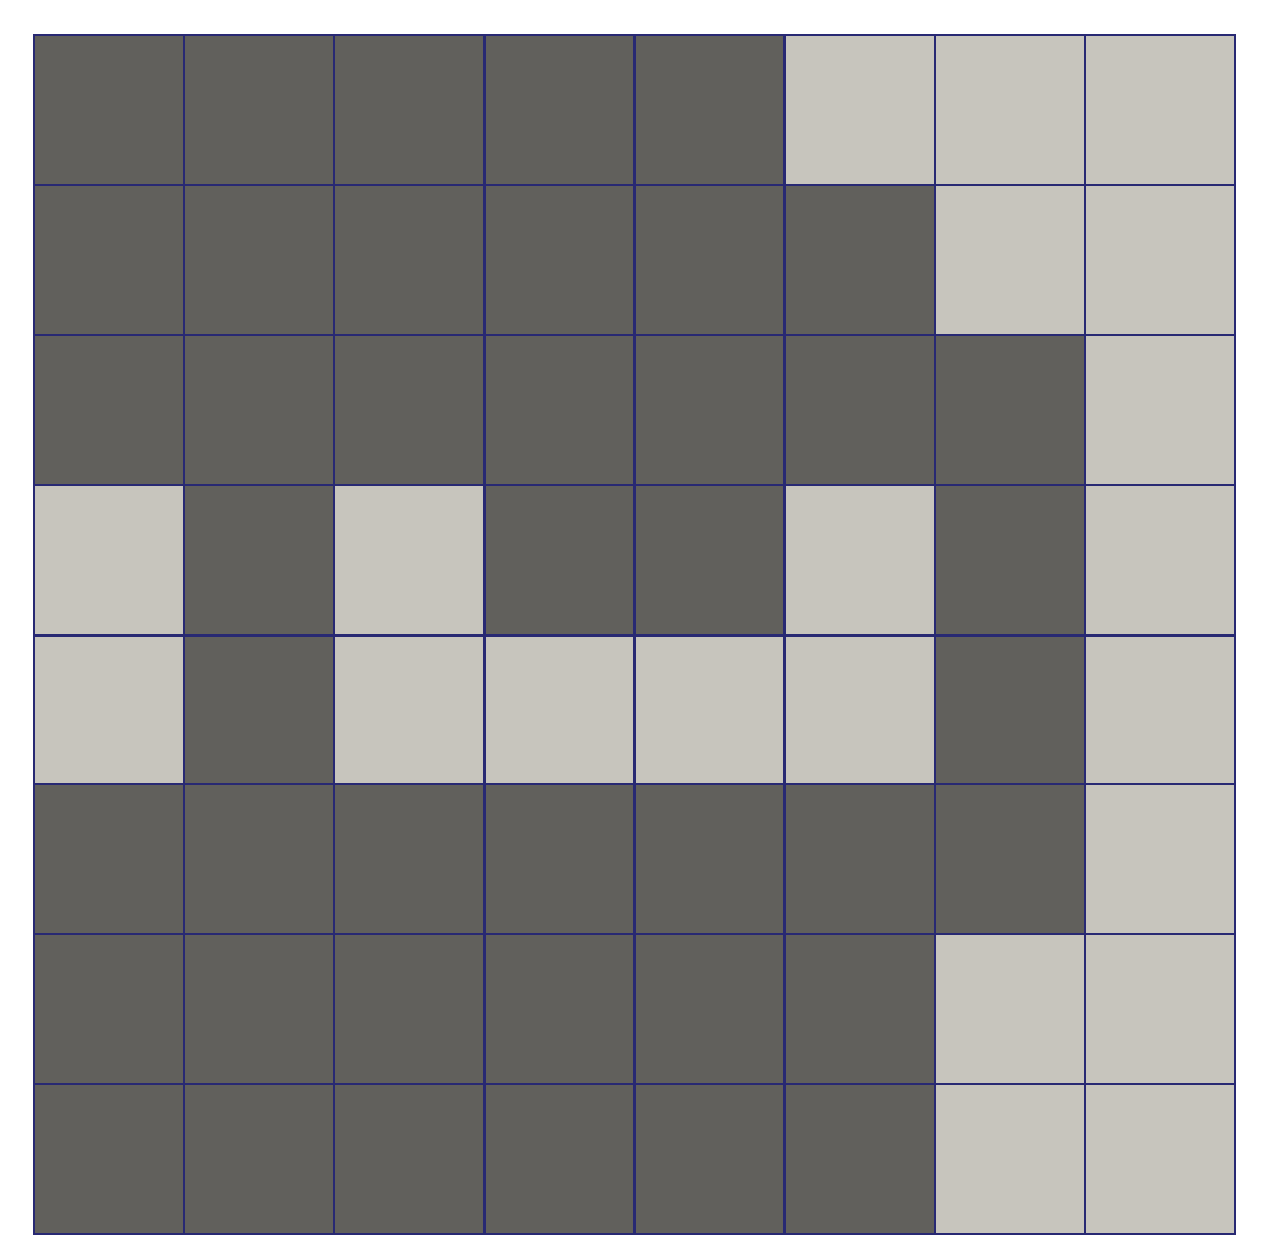
\includegraphics{adaptivity/images/adap_svm_train_my_cantilever_0.eps}
        }
    \end{subfigure}
    \begin{subfigure}[b]{0.49\linewidth}
        \scalebox{0.25}{
            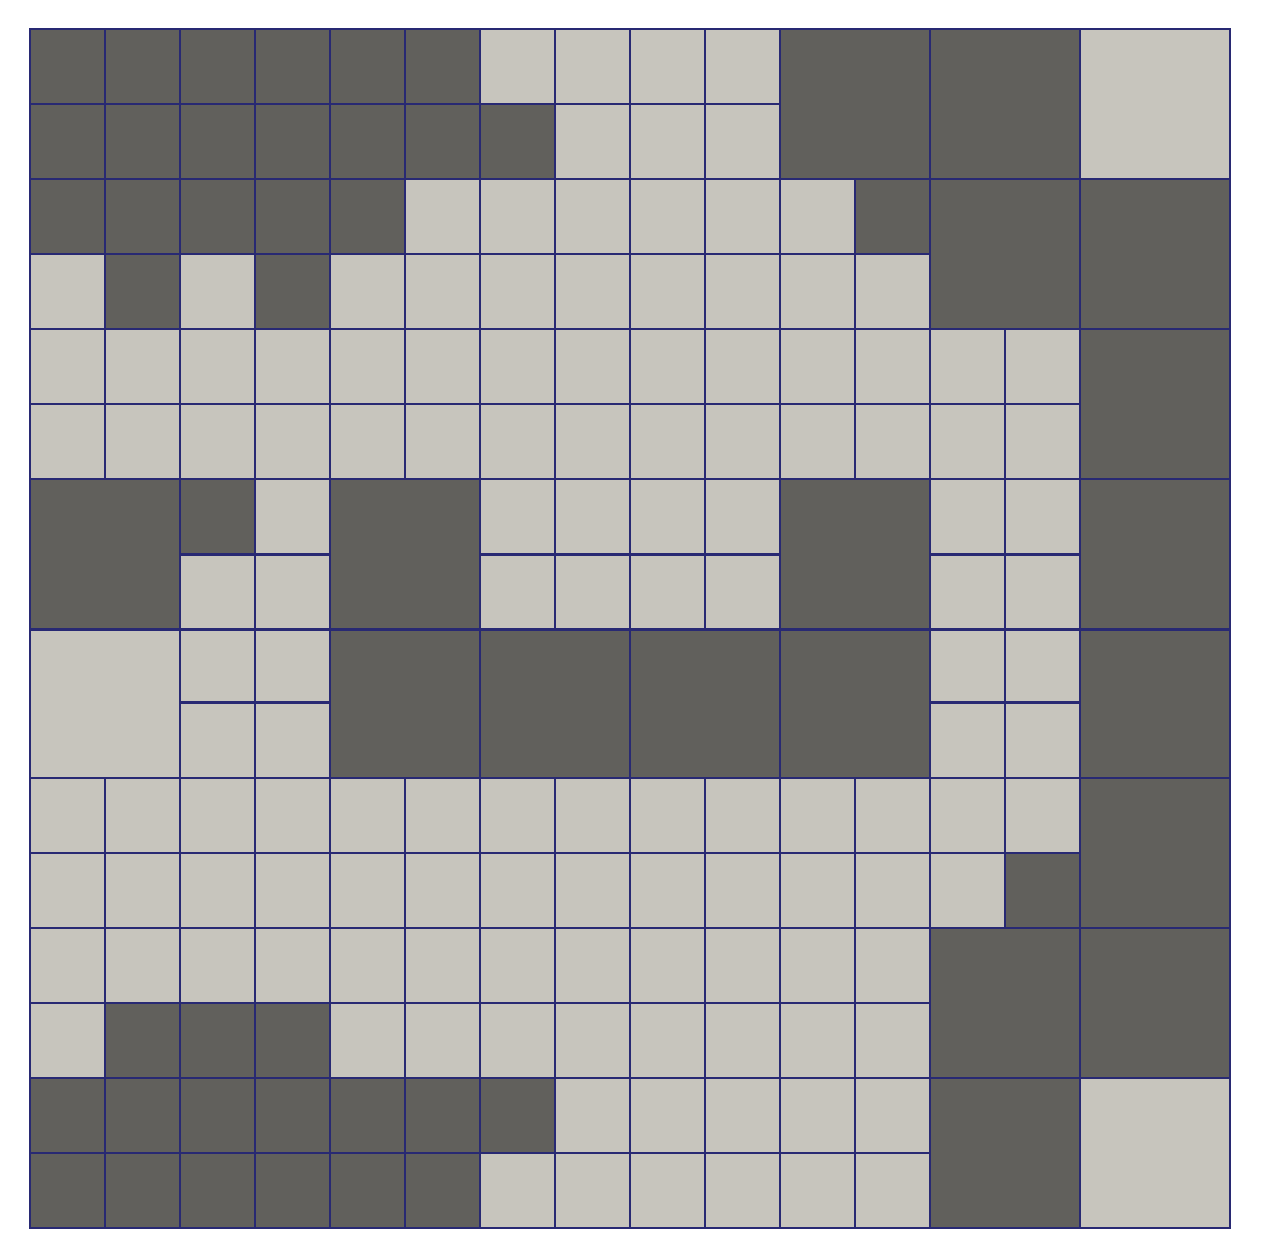
\includegraphics{adaptivity/images/adap_svm_train_my_cantilever_1.eps}
        }
    \end{subfigure}
    \caption[Training data for SVM]{Training data for SVM: Cells in black is marked as refined.}
    \label{adap_fig:svm_train_my}
\end{figure}
%
Criteria taken into consideration are: 
\begin{enumerate}
    \item Ratio of the area of the cell to the total area
    \item Minimal angle formed by the intersecting lines connected by scaling center and adjacent polygon vertexes
    \item Eigenvalue error indicator for displacement
    \item Eigenvalue error indicator for stress
\end{enumerate}
%
\subsection{Regularization for MLP}
\paragraph{Bagging}
\label{adp_sec:ml_bagging}
Bagging is a technique that utilize multiple models in order to increase the accuracy of the prediction \citep{Breiman1996}.
The principle of idea of that is simple: training multiple models separately and let them vote for the prediction.
It is adopted vastly in machine learning.
The idea behind the optimization technique is that different models often make different errors on the same test set.
Take a set of $k$ regression models for an example, error $\epsilon_i$ is made by each model on each example.
The errors are drawn from a zero-mean multivariate normal distribution with variances $E[\epsilon_i^2]$ = $\nu$ and covariances $E[\epsilon_i \epsilon_j]$=$c$.
As a result, the overall error determined by averaging of all models is $\frac{1}{k}\sum_i \epsilon_i$.
The expected squared error of the ensemble predictor is
\begin{equation}
    \begin{aligned}
    E[(\frac{1}{k} \sum_i \epsilon)^2] &=
    \frac{1}{k^2}[
        \sum_i (
            \epsilon_i^2 + \sum_{j\neq i}\epsilon_i \epsilon_j
        )
    ] \\
    &= \frac{1}{k}\nu + \frac{k-1}{k}c
    \end{aligned}
\end{equation}
%
The bagging technique does not help if the errors are highly correlated and $c=\nu$ as the mean squared error can reduce to $\nu$.
On the other hand, the effect of this technique may be significant if the errors are highly uncorrelated and $c=0$, in which situation the overall mean squared error becomes $\frac{1}{k}\nu$.
In other words, the overall mean squared error decreases linearly with the model size.
To conclude, the performance of this technique must not be worse than any of its individual model and a significant improvement can be expected if its members make independent errors.

\paragraph{}
There are several different methods to train ensemble.
For instance, each member of the ensemble can be trained with same training set but different algorithms or different training set with same algorithm.
The reuse of the same kind of models and algorithms is allowed thanks to the bagging.
The bagging technique used in the proposed method is constructing $k$ different training set.
Each training is built by sampling the original data set randomly.
In other words, each individual model may have some dataset which is not appear in any other models.
There is also some dataset are shared by multiple models.

\paragraph{}
Due to the large number of initialization parameter for a neural network, bagging technique can be extremely effective because the random selection of parameters such as initialized weight, mini-batches, hyper-parameters and so on leads to a different outcome even with the same training data.
The method is proved to be reliable and powerful for minimizing the generalization error.
Averaging dozens of models is widely adopted in those who won the machine learning contests and a recent example is Netflix Grand Price \citep{koren2009}.


\paragraph{Dropout}
Dropout \citep{JMLR:v15:srivastava14a} is another optimization approach used in the proposed method.
An effective but computationally cheap regularizing technique is provided.
Roughly speaking, the dropout can be regarded as one method to create different models in bagging described in Sec.~\ref{adp_sec:ml_bagging} by training multiple models.
One problem in bagging is that it could be impractical when each model is so large that the training can be computationally expensive in terms of time and space complexity.
Hence, the number of models used in ensembles tends to be in the range of $5$ and $10$ and the winner of ILSVRC \citep{DBLP:journals/corr/SzegedyLJSRAEVR14} used $6$ models.
As a comparison, dropout provides an cheap algorithm that can train and evaluate a large number of bagged ensemble.

\paragraph{}
In dropout, random hidden units are disabled during the training, which can be easily achieved by manually setting the weight to zero.
By doing so, the contribution of this hidden unit is ignored based on the fact that matrix production is used.
It can also be implemented by removing the unit completely from the network.
In bagging technique, $k$ different models with different training data are trained.
This is shared by the dropout as well, while dropout supports larger number of neural networks.
During the training process using dropout, a minibatch-based learning algorithm introduced in Sec.~\ref{lr_sec:ml_sgd} is used to make insignificant steps.
Whenever a sample is loaded into the minibatch, a random binary mask is applied to all of the inputs and hidden units in the network.
The probability a unit be disabled is independent from others and shall be determined from the user input as one of the hyperparameter.
In the proposed method, an input units has $20\%$ chance of being disabled and the number is $50\%$ for the hidden units.


\paragraph{}
More formally, assume that a mask vector $\mu$ specifies which units to include and $J(\theta,\mu)$ defines the cost of the model defined by parameters $\theta$ and mask $\mu$ \citep{Goodfellow-et-al-2016}.
After that, the training of the dropout becomes minimizing $E_\nu J(\theta,\mu)$.
The expectation may includes great number of terms while it could be possible to determine an unbiased estimation of its gradient by sampling values of $\mu$.

\paragraph{}
The training of the dropout is quite different to that of bagging.
Models use same parameters but different training data in bagging as shared parameters help to represent numerous number of models without occupying too many memory.
During the training using bagging, individual model is trained until convergence while during the training using dropout, most of the models are not explicitly trained.
That is because the number of the possible sub-network in dropout is too significant to finish the training within the lifetime of the universe.
Instead, only minor proportion are trained for a single step.
Parameter sharing guarantee that the remaining sub-networks are able to arrive at good settings.
The bagging algorithms are followed after that.
For instance, the training data used by individual model actually is sampled from the original training set.
Simple majority of the votes from all members are adopted to determine the prediction of the ensemble.
Although bagging and dropout does not require a explicitly probabilistic model, it is assumed that a probability distribution $p^{(i)}(y|x)$ will be the output.
The prediction of the ensemble is given by averaging all these distributions,
\begin{equation}
    \frac{1}{k} \sum_{i=1}^k (y|x)
\end{equation}
%
For dropout, individual model with a mask vector $\mu$ defines a probability distribution $p(y|x, \mu)$.
The arithmetic mean over all masks is given by
\begin{equation}
    \sum_\mu p(\mu) p(y|x, \mu)
    \label{adap_eq:ml_dropout_sum}
\end{equation}
%
where $p(\mu)$ is the probability distribution used to sample $\mu$ during the training.
Since numerous number of terms are involved in the summation, it could be difficult to calculate Eq.~\ref{adap_eq:ml_dropout_sum} without simplification.
However, a deep neural network do not allow such simplification.
Instead, it is possible to approximate the simplification with sampling by calculate the mean value from many masks.
It is suggested that around $15$ masks are able to provide satisfactory performance \citep{Goodfellow-et-al-2016}

\paragraph{}
Yet, the existence of a better approach allows the determination of a satisfactory approximation to the predictions of the ensemble at the cost of one forward propagation.
It can be achieved by adopting geometric mean instead of the arithmetic mean of the ensemble member's predicted distributions \citep{WardeFarley2014SelfinformedNN}.
However, using the geometric mean instead of the arithmetic mean leads to the result which is not guaranteed to be a probability distribution.
In order to enforce a probability distribution as the result, the requirement that all sub-models must assign a non-zero probability to all events is imposed.
After that, the resulted distribution is normalized again.
The unnormalized probability distribution from geometric mean is:
\begin{equation}
    \tilde{p}_{ensemble}(y|x) = 2^d \sqrt{\prod_\mu p(y|x,\mu)}
\end{equation}
%
where $d$ is the number of units that my be dropped.
To simplify the presentation, a uniform distribution over $\mu$ is adopted.
But it should be noted that non-uniform distributions can be treated as well.
Eq.~\ref{adap_eq:ml_renormalize} need to be performed on the ensemble in order to determine the prediction
\begin{equation}
    p_{ensemble}(y|x) = \frac{
        \tilde{p}_{ensemble}(y|x)
    }{
        \sum_{y^\prime} \tilde{p}_{ensemble}(y^\prime|x)
    }
    \label{adap_eq:ml_renormalize}
\end{equation}
%
The key idea behind the dropout is to approximate $p_{ensemble}$ by calculating $p(y|x)$ in one model \citep{hinton2012}.
The aim of this improvement is to capture the correct output from that unit.
It is called weight scaling inference rule which shows outstanding performance empirically.
\paragraph{}
Since an inclusion probability of $\frac{1}{2}$ is widely adopted, the weight scaling rule tends to half the weights after training.
The model is used as usual after that.
It can also be achieved by multiplying the states of the units by $2$ during training.
Both of these two methods are to narrow the difference between the expected total input to a unit at test time and that at the training when approximately half of the hidden units are dropped.
For those models without nonlinear hidden units, the weight scaling inference rule gives exact result.
For instance, a softmax regression classifier with $n$ input variables represented by the vector $v$ is considered:
\begin{equation}
    P(y=y|v)=softmax(W^Tv+b)_y
\end{equation}
%
They can be indexed into the family of sub-models by element-wise multiplication of the input with a binary vector $d$:
\begin{equation}
    P(y=y|v;d) = softmax(W^T(d \odot v)+b)_y
\end{equation}


\subsubsection{Indicator used in adaptivity}
\paragraph{}
All terms used in the performance indicators in machine learning are introduced in Sec.~\ref{lr_ml:indicators}
The balance of the indicators is highly dependent on classifiers' objective.
Take the spam detector for an example, a false positive can be more dangerous than a false negative as an important e-mail being marked as spam can be a disaster.
While in adaptivity, there may be no favour over either of them.
It is because the refinement of a cell with lower error or leaving a cell with higher error unrefined may not produce significant influence on the final result.
As a result, F1 score can be the most important indicator as it takes both recall rate and precision into consideration.


\subsection{Result}
\paragraph{}
All training data are standardized by Eq.~\ref{adap_eq:svm_standardized} where $\overline{x}$ and $\sigma$ is the mean and standard deviation of the data.
It makes features in training data have zero means and unit variance.
Cells that need to be refined are labeled as $1$ and the rest are labeled as $0$.
Radial basis function with $\sigma=0.7624$ is adopted as kernel function in SVM.
    \begin{equation}
        x^\prime = \frac{x-\overline{x}}{\sigma}
        \label{adap_eq:svm_standardized}
    \end{equation}
Half of the training data ($320$ out of $640$) are used to train the model and the reset are used for cross validation.
Different class weights are set for testing different performance in regard to all indicators in Fig.~\ref{adap_fig:svm_performance_0}.
\begin{figure}[h!]
    \centering
    \scalebox{0.3}{
        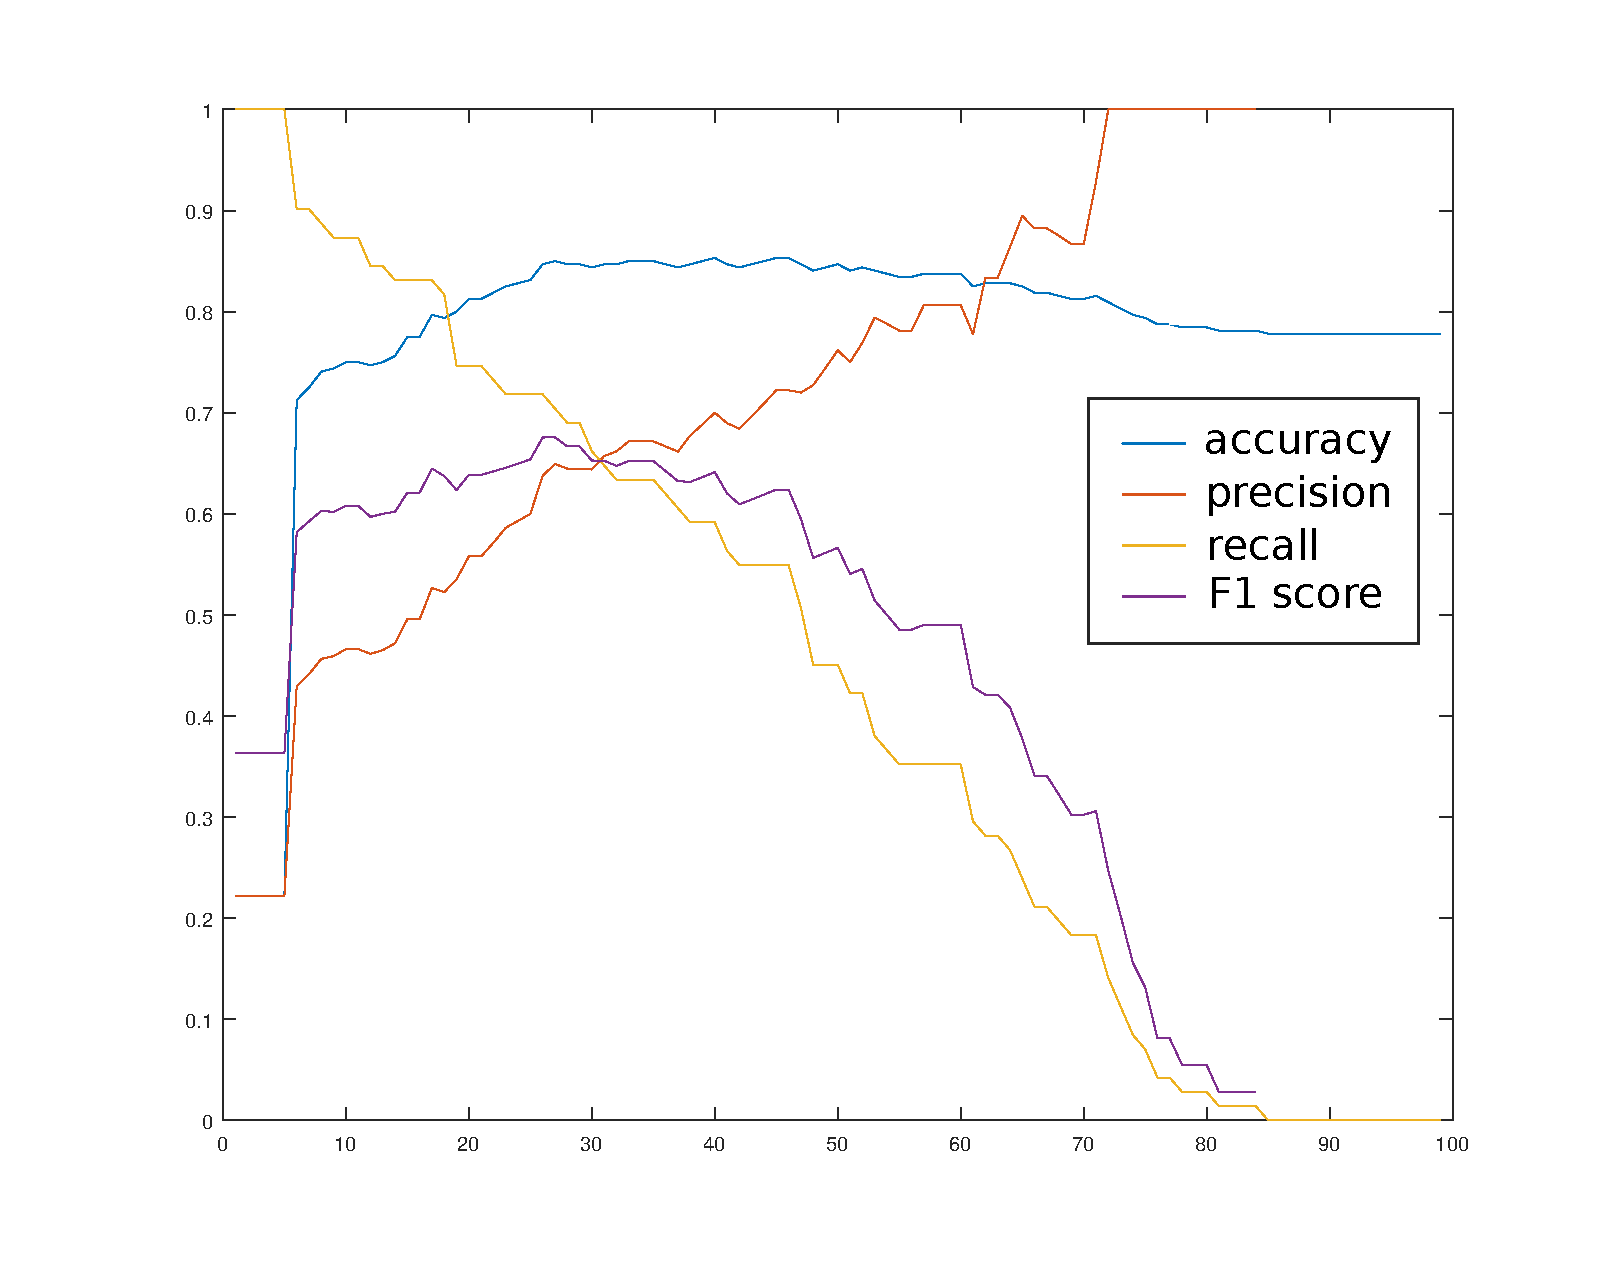
\includegraphics{adaptivity/images/svm_performance_0.eps}
    }
    \caption{Accuracy, precision, recall rate and F1 score vs different class weight}
    \label{adap_fig:svm_performance_0}
\end{figure}
%
A class weight is a vector that influence the predication directly.
The model will calculate the probability for each classification based on the input and the one with higher probability will be chosen as the result in default situation.
Change class weight to $1:2$ will force the model to choose first class when its probability is higher than $66.67\%$ instead of $50\%$.
A class weight of $3:7$ was chosen from Fig.~\ref{adap_fig:svm_performance_0} to guarantee a balance between precision and recall rate.
The corresponding result is listed in Tab.~\ref{adap_tab:svm_result}.
\begin{table}[h!]
    \centering
    \caption{Result of cross validation}
    \begin{tabular}{cc}
        \toprule
        Accuracy    &   84.38\%    \\
        Precision   &   64.38\%     \\
        Recall rate &   66.20\%     \\
        F1 score    &   65.28\%     \\
        \bottomrule
    \end{tabular}
    \label{adap_tab:svm_result}
\end{table}
%  compare auc
\pagebreak


\section{Merging triangle}
\label{adap_merge_triangle}

\paragraph{}
% why
Due to the property of the SBFEM, first order triangle element will result identical eigenvalues of one.
Under this circumstances, the displacement, nodal forces and energy using eigenvalues failed as the they are always equal to the order of the shape function, one.
As a consequence, the triangular elements shall be merged with their neighbours to form a larger polygon.
Besides, due to the fact that triangular elements are formed by cutting with the geometric boundary, triangular elements have a higher chance to be obtuse triangles, which lead to poor quality mesh.
As a result, merging triangle can help to improve the mesh quality as well.

\begin{figure}[!ht]
    \begin{subfigure}[b]{0.5\linewidth}
        \centering
        \scalebox{0.8}{
            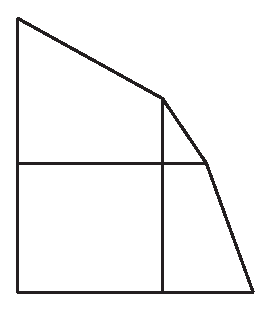
\includegraphics{adaptivity/images/adap_mt_int_before.eps}
        }
    \caption{before}
    \end{subfigure}
    \begin{subfigure}[b]{0.5\linewidth}
        \centering
        \scalebox{0.8}{
            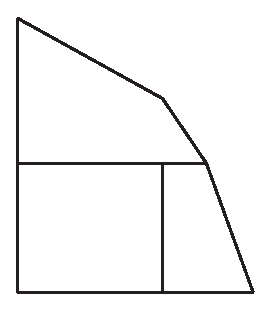
\includegraphics{adaptivity/images/adap_mt_int_after.eps}
        }
    \caption{after}
    \end{subfigure}
    \caption[Merging triangle]{Merging triangle}
    \label{adap_fig:mt_introduction}
\end{figure}

\paragraph{}
There are three steps to perform a triangle merging.
\begin{enumerate}
    \item Finding the polygon to merge with
    \item Merging triangle with the polygon
    \item Adjusting scaling center
\end{enumerate}

\paragraph{}
The first step of merging triangle is to find the appropriate cell to merge with.
Generally speaking, there will be two or three candidate as shown in Fig.~\ref{adap_fig:mt_choose}
Since triangular elements are always generated by cut by the boundary, one of these possibility must contain the other part of the origin cell (cell 2 in Fig.~\ref{adap_fig:mt_choose}).
However, as the cut by the boundary is necessary, undo the cut could be meaningless.
As a result, this possibility can be ignored.
If there are two remaining possibility as in Fig.~\ref{adap_fig:mt_choose_3p}, the triangle will be merged with the cell that share the longer edge with it.
Triangle $0$ in Fig.~\ref{adap_fig:mt_choose_3p} will be merged with cell $1$ instead of $3$ because $AB > AC$.
It is because of the following reason.
Take Fig.~\ref{adap_fig:mt_choose_3p} as an example, edge $AD$ will be extended to $DC$ if triangle $0$ is merged with polygon $1$.
So merging triangle with the polygon that share a longer edge with means the polygon will less elongated and leads to a better mesh quality.
Furthermore, the polygon to merge with the triangle must have the same material property with the triangular element, otherwise they shall not be combined together.
In some extreme case, the merging triangle may not be possible as the triangular element itself fill the whole region with a specific material property.
A reasonable selection of hyperparameter in generating mesh can prevent it from happening.

\begin{figure}[!ht]    
    \begin{subfigure}[b]{0.5\linewidth}
        \centering
        \scalebox{0.8}{
            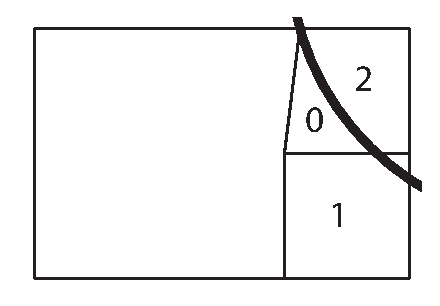
\includegraphics{adaptivity/images/adap_mt_choose_2pos}
        }
        \caption{Two possibility}
    \end{subfigure}
    \begin{subfigure}[b]{0.5\linewidth}
        \centering
        \scalebox{0.8}{
            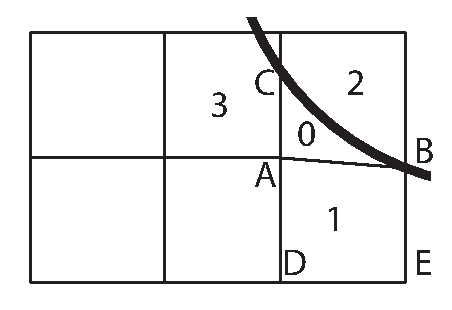
\includegraphics{adaptivity/images/adap_mt_choose_3pos}
        }
        \caption{Three possibility}
        \label{adap_fig:mt_choose_3p}
    \end{subfigure}    
    \caption[Choose the cell to merge with]{Choose the cell to merge with}
    \label{adap_fig:mt_choose}
\end{figure}

\paragraph{}
The second step which is merging the triangular element with the polygon is straightforward.
It should be noted that one point (point $A$ in Fig.~\ref{adap_fig:mt_choose_3p}) is possible to be removed.
A calculation of the distance from point $A$ to line $CD$ can always help to determine whether the point can be removed or not.

\paragraph{}
% centroid
The last step is to find the scaling center for the new generated polygon.
Due to the fact that the merged polygon is very unlikely to be a polygon that looks like a square, taking the mean of all vertexes as the scaling center may not be a good idea.
Calculating the geometric center of the polygon and take it as the scaling center may be an optimized solution.
The centroid $C$ of a polygon with $n$ points $\{(x_1,y_1),(x_2,y_2),\dots,(x_n,y_n)\}$ can be calculated as
\begin{equation}
    \begin{aligned}
        C_x &= \frac{1}{6A} \sum_{i=0}^{n-1}\left(
            x_i + x_{i+1}    
        \right) \left(
            x_i y_{i+1} - x_{i+1} y_i
        \right) \\
        C_y &= \frac{1}{6A} \sum_{i=0}^{n-1}\left(
            y_i + y_{i+1}    
        \right) \left(
            x_i y_{i+1} - x_{i+1} y_i
        \right)
    \end{aligned}
\end{equation}
where $A$ stands for the area of the polygon.

\paragraph{}
% concave polygon
However, centroid of a concave polygon may be located at the outside of the polygon, result in an invalid scaling center.
Consequently, special treatment is need to adjust the scaling center.
If the mesh in the previous steps are correct, there should not be more than one reflexive angle in the polygon.
So the vertex of that reflexive angle must be found first.
It can be easily done by check the cross product between any two adjacent edges as vectors and find the only one whose sign is different with others.
An angle bisector then is drawn and the intersection between it with the edge of the polygon will be recorded (point $B$ in Fig.~\ref{adap_fig:mt_concave_sc}).
The mid point of line $AB$ will be select as the scaling center of that concave polygon.

\begin{figure}[!ht]
    \centering
    \scalebox{0.8}{
        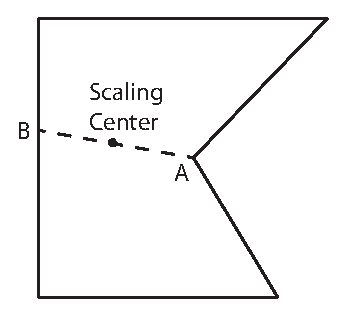
\includegraphics{adaptivity/images/adap_mt_concave_sc.eps}
    }
    \caption[Scaling center for concave polygon]{Scaling center for concave polygon}
    \label{adap_fig:mt_concave_sc}
\end{figure}





\section{Matrix representation of NURBS Curves}
\label{adap_sec_mrep2d}
\subsection{Implicit Matrix Representation}
\label{adap_sec:mrep}
\paragraph{} 
Matrix representation of a parameterized algebraic curve allows an easy way to calculate the intersection between it with another curve and find the corresponding parameter based on the given point on the curve.
For an algebraic curve $t \in \mathbf{R}^1 \xrightarrow{\phi} \left( \frac{f_1(t)}{f_0(t)}, \frac{f_2(t)}{f_0(t)},\frac{f_3(t)}{f_0(t)} \right) \in \mathbf{R}^3$, $f_0,f_1,f_2$ and $f_3$ are polynomials functions in parameter $t$ with degree $\leq p$.
The procedure of constructing the matrix representation for NURBS curves are explained detail in \citep{Laurent2014}.
\paragraph{}
The aim of this method is to find 4-tuples of polynomials\\
$\left( g_0(t),g_1(t),g_2(t),g_3(t) \right)$ with order $v$ so that
\begin{equation}
    \sum_{i=0}^3 g_i(t) f_i(t) \equiv 0
    \label{adap_eq_mRep_eq0}
\end{equation}
%
who is a vector space and one of its bases can be:
\begin{equation}
    \mathbf{L_j}(t,X,Y,Z) = g_0(t) + Xg_1(t) + Yg_2(t) + Zg_3(t)
    \label{adap:eq:mrep_eq1}
\end{equation}
Since $g$ is also a polynomial based function, it can be expressed in the vector space with a set of bases of $\left\{\psi_1(t), \psi_2(t), \dots, \psi_{m_v}(t) \right\}$ and the bases $\mathbf{L_j}$ can be expressed as
    \begin{equation}
        \begin{aligned}
            \mathbf{L_j} &= \sum^{m_v}_{i=1}\left( \lambda_{0,i}^{(j)} + \lambda_{1,i}^{(j)}X + \lambda_{2,i}^{(j)}Y + \lambda_{3,i}^{(j)}Z\right)\psi_i(t)\\
        & = \sum_{i=1}^{m_v} \Lambda_{i,j}(X,Y,Z)\psi_i(t)
        \end{aligned}
    \end{equation}
%
Finally, a matrix which represents the mapping of $\phi$ in a $m_v \times r_v$-matrix $\mathbf{M_v}$ with order $v$
    \begin{equation}
        \mathbf{M_v}(\phi) = 
        \begin{bmatrix}
        \Lambda_{1,1} & \Lambda_{1,2} & \dots & \Lambda_{1,r_v} \\ 
        \Lambda_{2,1} & \Lambda_{2,2} & \dots & \Lambda_{2,r_v} \\ 
        \vdots 		  & \vdots 		  &  	  &\vdots			\\
        \Lambda_{m_v,1}&\Lambda_{m_v,2}&\dots &\Lambda_{m_v,r_v}
        \end{bmatrix}
    \end{equation}



%=====================================================================================================================%
\subsection{Matrix Representation for Rational Bézier Curves}
An rational bézier curves can be defined by 
\begin{equation}
	\phi:t\in \mathbf{R}\rightarrow \frac{\sum_{i=0}^pw_i\mathbf{P}_iB_i^p(t) }{\sum_{i=0}^pw_iB_i^p(t)}
\end{equation}
where
\begin{equation}
    B_i^p(t) = \mathbf{C}_i^dt^i(1-t)^{d-i}
    \label{adap_eq_mrep_bbasis}
\end{equation}
%
The aim is to find a matrix whose vector is in the form of
\begin{equation}
    [\alpha] =
    \begin{bmatrix}
        \alpha_{0,0} & \alpha_{0,1}&  \dots&  \alpha_{0,v} & \alpha_{1,0} & \dots & \alpha_{3,v} 
    \end{bmatrix}^T
\end{equation}
%
where $g_j(t)$ in Eq.~\ref{adap:eq:mrep_eq1} can be expressed as
\begin{equation}
    g_j(t) = \sum_{i=0}^v \alpha_{j,i}B_i^v(t)
\end{equation}
%
Based on Eq.~\eqref{adap_eq_mRep_eq0}, it can be concluded that $\mathbf{R}\times\left[\alpha\right]=0$
\begin{equation}
    \mathbf{R} = 
    \begin{bmatrix}
        B_0^v(t)f_0(t) & \dots & B_v^v(t)f_0(t) & B_0^v(t)f_1(t) & \dots & B_v^v(t)f_3(t)
    \end{bmatrix}
\end{equation}
%
By having another set of basis $\mathbf{L_v}$ and the transformation matrix $\mathbf{S}$ so that $\mathbf{L_vS}=\mathbf{R}$ where
\begin{equation}
    \mathbf{L_v}=
    \begin{bmatrix}
        B_0^{v+d}(t) & B_1^{v+d}(t) & \dots & B_{v+d}^{v+d}(t)
    \end{bmatrix}
\end{equation}
%
This leads to
\begin{equation}
    \begin{bmatrix}
        B_0^{v+d}(t) & B_1^{v+d}(t) & \dots & B_{v+d}^{v+d}(t)
    \end{bmatrix}\times \mathbf{S}\times\left[\alpha\right] = R\times\left[\alpha\right] = 0
\end{equation}
which indicates $\left[ \alpha\right]$ is in the null space of $\mathbf{S}$

After substituting $f(t) = \sum_{i=0}^dc_iB_i^d(t)$ into $\mathbf{R}$, the following can be deduced
\begin{equation}
    B_j^v(t)f(t) =  \sum_{i=0}^dc_iB_i^d(t)B_j^v(t) =\sum_{i=0}^d \frac{\mathbf{C}^v_j\mathbf{C}^d_i}{\mathbf{C}^{d+v}_{i+j}}c_i B_{i+j}^{d+v}(t)
\end{equation}
%
which indicates that
\begin{equation}
    \mathbf{S}_{i+j,j} = \frac{\mathbf{C}^v_j\mathbf{C}^d_i}{\mathbf{C}^{d+v}_{i+j}}c_i
\end{equation}
%
Finally, the null space of $\mathbf{S_v}$, $\mathbf{M_v}$ is the matrix representation of the rational bézier curve.



%=====================================================================================================================%
\subsection{Intersection}
The calculation of the intersection is described in detail in \citep{Buse2010, Ba2009}.
All intersections can be calculated at once by using matrix representation of the algebraic curve.
\paragraph{} 
Given a rational curve/surface $C1$
\begin{equation}
    \mathbf{P}^1 \xrightarrow{\phi_1} \mathbf{P}^n: (u,v) \rightarrow(f_0,f_1,f_2,f_3)(u,v)
\end{equation}
%
the aim is to find the intersection between it with another rational curve $C2$ via matrix representation
\begin{equation}
    \mathbf{P}^1 \xrightarrow{\phi_2} \mathbf{P}^n: (t) \rightarrow(g_0,g_1,g_2,g_3)(t)
\end{equation}
%
is to find
\begin{equation}
    \mathbf{M}_{v1}(\phi_2(t) = 0
\end{equation}
%
which leads to
\begin{equation}
    \mathbf{M_0}g_0 + \mathbf{M_1}g_1 + \mathbf{M_2}g_2 + \mathbf{M_3}g_3 = 0
    \label{mRep_intec_base}
\end{equation}
%
By knowing $g_n$ is a polynomial function with order $p$, Eq.~\eqref{mRep_intec_base} can be rearranged as
\begin{equation}
    \mathbf{M}(t) = \sum_{i=0}^p \mathbf{M_i}t^i
\end{equation}
%
After that, the generalized companion $q \times p$-matrices $A, B$ with rank $\rho$ are introduced
\begin{equation}
    A = 
    \begin{bmatrix}
        0		&I 		&\dots 		&\dots 		&0 		\\
        0 		&0 		&I 			&\dots 		&0 		\\
        \vdots 	&\vdots &\vdots 	&\vdots 	&\vdots \\
        0 		&0 		&\dots		&\dots 		&I 		\\
        M_0^t 	&M_1^t 	&\dots 		&\dots 		&M_{d-1}^t
    \end{bmatrix}
\end{equation}
%
\begin{equation}
    B = 
    \begin{bmatrix}
        I 		&0 		&\dots 		&\dots 		&0 		\\
        0 		&I 		&0 			&\dots 		&0 		\\
        \vdots 	&\vdots &\vdots 	&\vdots 	&\vdots \\
        0 		&0 		&\dots 		&I 			&0 		\\
        0 		&0 		&\dots 		&\dots 		&-M_d^t \\		
    \end{bmatrix}
\end{equation}
%
Before the eigenvalues are calculated, the regular part of a non-square pencil of the matrices shall be extracted first which is done by the following step
%
\paragraph{Step 1}
Transform $B$ into its column echelon form:
SVD-decomposition is adopted to perform the task.
\begin{equation}
\begin{aligned}
    B_1 = BV_0 = [\underbrace{B_{1,1}}_{\rho} |\underbrace{0}_{q-\rho}]	\\
    A_1 = AV_0 = [\underbrace{A_{1,1}}_{\rho} |\underbrace{A_{1,2}}_{q-\rho}]
\end{aligned}
\end{equation}
%
\paragraph{Step 2}
Transform $A_{1,2}$ into its row echelon form:
\begin{equation}
    U_1A_{1,2} = 
    \begin{bmatrix}
        \underline{A^\prime_{1,2}}\\
        0
    \end{bmatrix}
\end{equation}
%
where $A^\prime_{1,2}$ is in full row rank.\\
At the end of step 2, matrix $A$ and $B$ can be represented as
\begin{equation}
\begin{aligned}
    A^\prime_1 &=
    \begin{bmatrix}
        A^\prime_{1,1} & A^\prime_{1,2} \\
        \cmidrule(lr){1-2}
        A_2 & 0
    \end{bmatrix}\\
    B^\prime_1 &=
    \begin{bmatrix}
        B^\prime_{1,1} & 0\\
        \cmidrule(lr){1-2}
        B_2 & 0
    \end{bmatrix}
\end{aligned}
\end{equation}
where $A^\prime_{1,2}$ has full row rank\\
$
\begin{bmatrix}
\underline{B^\prime_{1,1}}\\
B_2
\end{bmatrix}
$ has full column rank\\
$
\begin{bmatrix}
\underline{B^\prime_{1,1}}\\
B_2
\end{bmatrix}
$ 
and $B_2$ are in echelon form
\paragraph{}
$A_2$ and $B_2$ will be the new $A$ and $B$ matrices for next iteration until $B$ has full rank.
If $B$ has full row rank but not full rank, $A=A^T$ and $B=B^T$ are conducted.
\paragraph{}
After these processes, $A$ and $B$ become two square matrices and $B$ is invertible so that the solution for the intersection parameter $t$ can be determined from the eigenvalue of the matrix $AB^{-1}$
\paragraph{}
However, the method may fail when the intersection is under the case where nearly tangential geometric conditions happens and return two empty matrices.
It is addressed by adding another step after extracting the real part of the $A$ and $B$ if the results are empty matrices\citep{Shen2016}.
If the input matrix $A$ and $B$ are not in full row rank or full column rank, it is considered that $C1 \cap C2 = C2$.
If the input matrix $A$ and $B$ are in full row rank or full column rank, a rank $m$ square sub-pencil is extracted assuming $A$ and $B$ have a rank of $m$.
Then the eigenvalues yield the intersections.



\section{Numerical examples}
% ansys, 12543*2 2nd order 4.92747
% ansys(1st)
% 100*2 - 4.82274
% 361*2 - 4.89143 
% 1369*2 -4.91566
% 5328*2 -4.92411
% err_a1 = abs([4.82274,4.89143,4.91566,4.92411]-4.92747)/4.92747; dof_a1 = [100,361,1369,5328]*2; polyfit(log(dof_a1), log(err_a1),1)


% ansys(2nd)
% 133*2 - 4.88648
% 481*2 - 4.91409
% 1825*2 - 4.92356
% 7105*2 -  4.92685
% err_a2 = abs([4.88648,4.91409,4.92356,4.92685]-4.92747)/4.92747; dof_a2 = [133,481,1825,7105]*2; polyfit(log(dof_a2),log(err_a2),1)

% svm
% 162 - 4.82
% 426 - 4.8945
% 992 - 4.9131
% 1780 - 4.9175
% 2614 - 4.9208
% err = abs([4.82,4.8945,4.9131,4.9175,4.9208] - 4.92747)/4.92747; dof=[162,426,992,1780,2614]; polyfit(log(dof),log(err),1)

% mlp
% 162-4.82
% 496-4.8884
% 1014-4.9090
% 1202-4.9151
% 3146-4.9226
% err = abs([4.82,4.8842,4.9060,4.9180,4.9226] - 4.92747)/4.92747; dof=[162,420,808,1484,3146]; polyfit(log(dof),log(err),1)

\subsection{Short cantilever beam}
\paragraph{}
A two-dimensional short cantilever beam subjected to a uniformly distributed load at the top is examined as shown in Fig.~\ref{adp_fig:ex_cantilever_beam_geo_bc}.
    \begin{figure}[h!]
    \centering
        \scalebox{0.5}{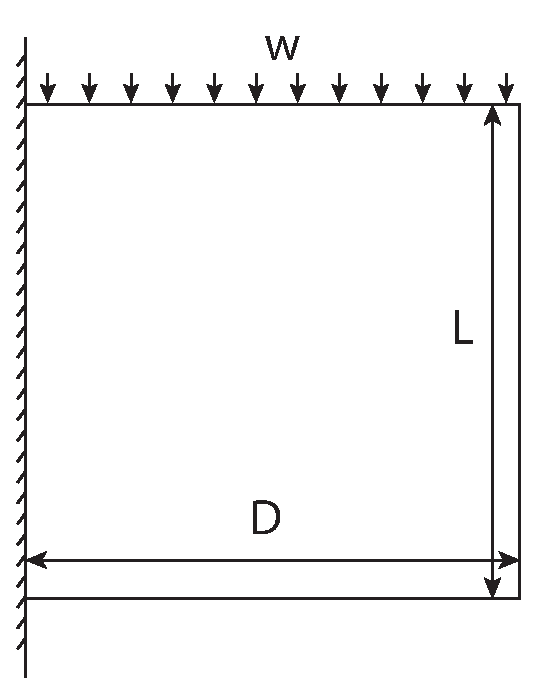
\includegraphics{adaptivity/ex_images/ex_short_cant_geo_bc.eps}}
        \caption{ Short cantilever beam: Geometry and boundary conditions.}
        \label{adp_fig:ex_cantilever_beam_geo_bc}
    \end{figure}

The geometry is: length $L = \SI{1}{\meter} $, height $ D = \SI{1}{\meter} $.
The material properties are: Young’s modulus $ E = \SI{20}{\newton \per \meter^2} $ , Poisson’s ratio $ \nu =0.3 $.
The uniformly distributed load is $w = \SI{10}{\newton \per \meter} $.
Plane stress condition is assumed.

The reference strain energy of \SI{4.02079}{\joule} is determined by the help of the ANSYS.
In the ANSYS, a mesh with $17930$ DOF using 2 \textsuperscript{nd} order plane element $183$ is used to calculate the result.

Due to the fact that the geometry of the cantilever beam can be described by four points and four straight lines, drawing in AutoCAD may not be necessary.
As a result, the input geometry is defined manually.


\paragraph{}
The numerical convergence of the the relative error in the energy norm is shown in Fig.~\ref{adap_fig:ex_short_cantilever_convergence}.
It can be observed that data mining based adaptive SBFEM yields superior convergence rate when compared to the result calculated in ANSYS.

\begin{figure}[h!]
    \centering
    \scalebox{0.5}{
        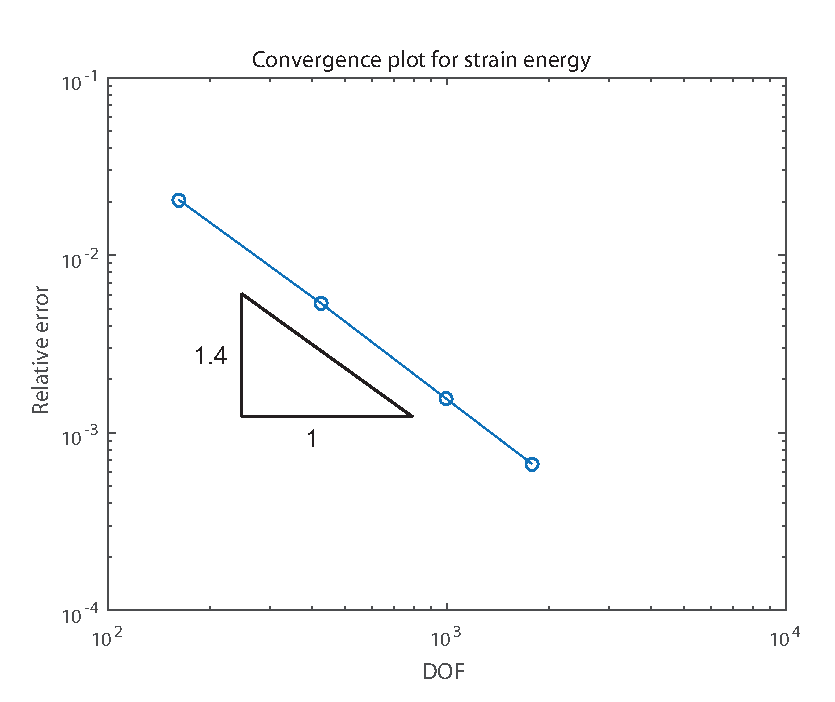
\includegraphics{adaptivity/ex_images/ex_short_cantilever_conv.eps}
    }
    \caption{the relative error in the energy norm}
    \label{adap_fig:ex_short_cantilever_convergence}
\end{figure}

Corresponding mesh development are plotted in Fig.~\ref{adap_fig:ex_short_cantilever_mesh_develpment} (SBFEM 1\textup{st} order element) and Fig.~\ref{adap_fig:ex_short_cantilever_mesh_develpment_ansys} (ANSYS 9-node quadrilateral element).
Stress contour plotted in ANSYS using 9-node quadrilateral elements (17930 DOFs) are shown in Fig.~\ref{adap_fig:ex_chole_stress_ansys}
\begin{figure}[h!]
\centering
    \begin{subfigure}[b]{0.4\linewidth}
        \centering
        \scalebox{0.25}{
            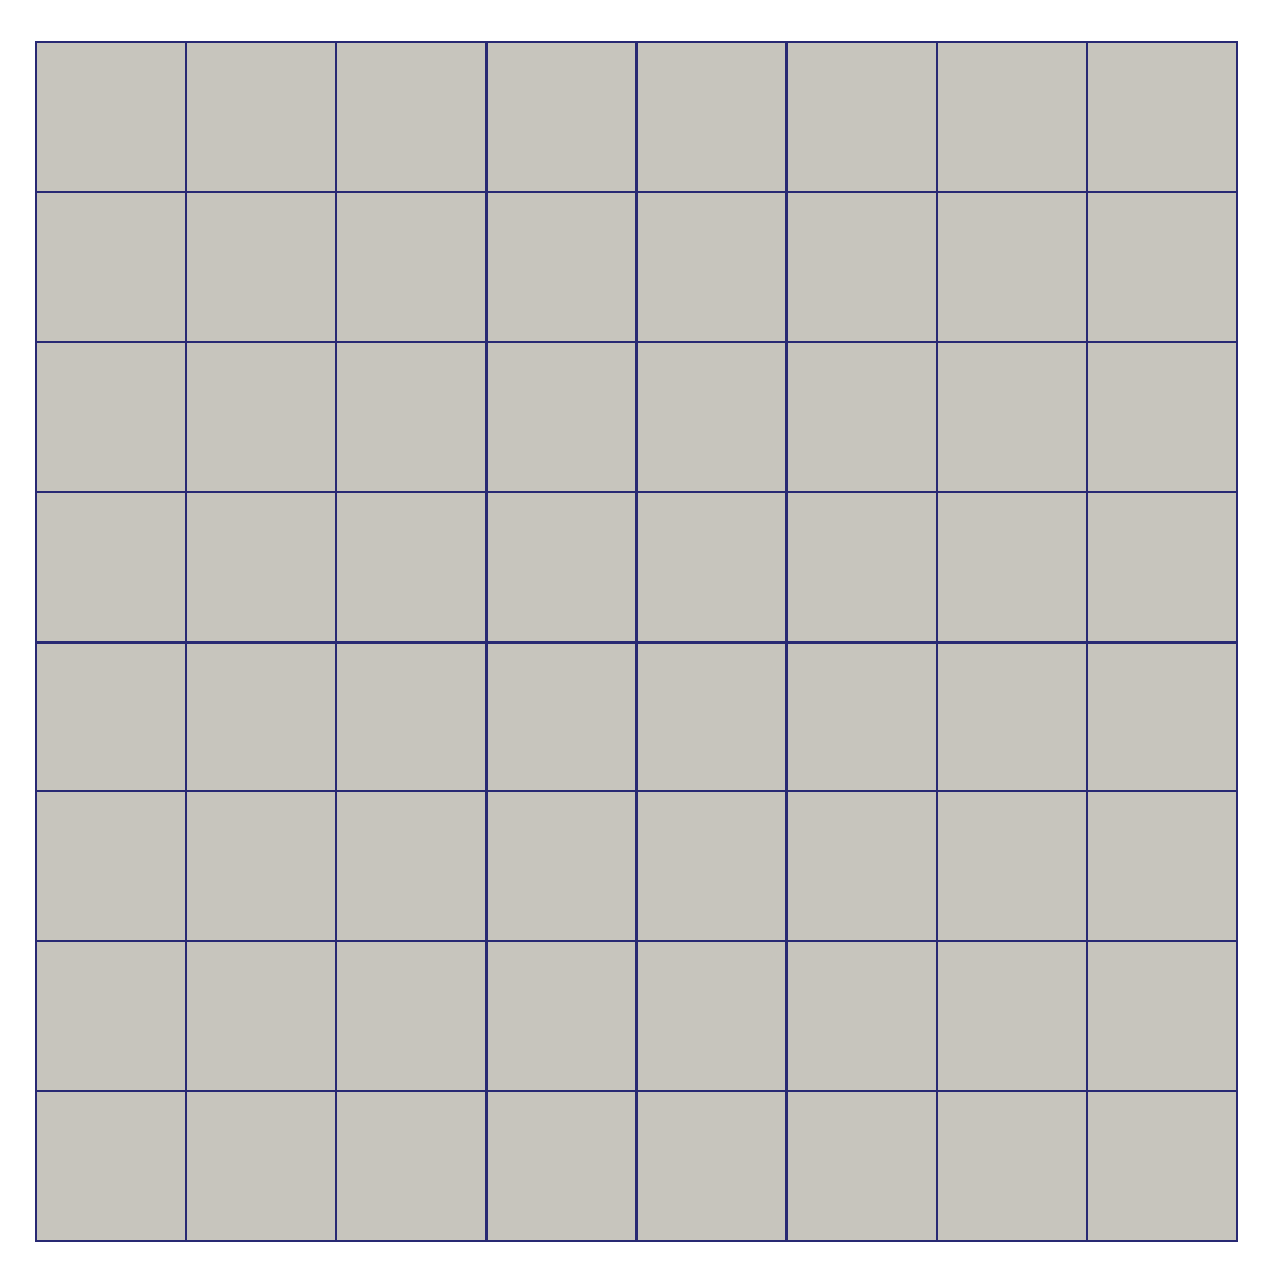
\includegraphics{adaptivity/ex_images/ex_short_cantilever_mesh_162.eps}
        }
        \caption{Initial mesh (162 DOF)}
    \end{subfigure}
    \begin{subfigure}[b]{0.4\linewidth}
        \centering
        \scalebox{0.25}{
            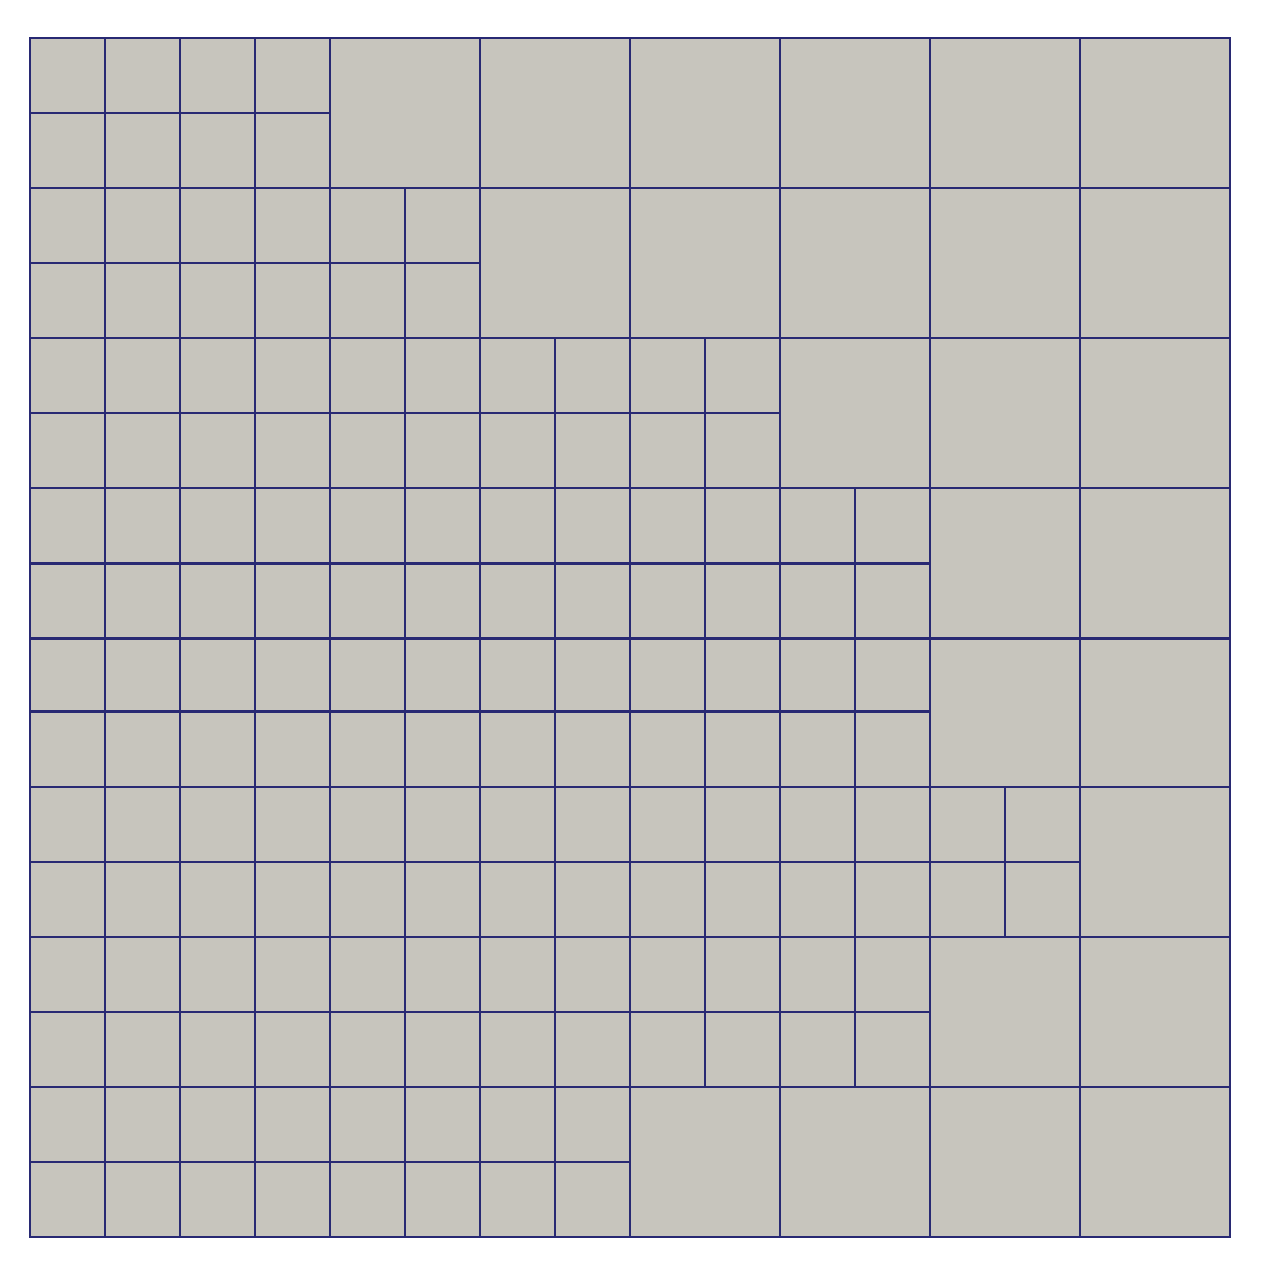
\includegraphics{adaptivity/ex_images/ex_short_cantilever_mesh_462.eps}
        }
        \caption{1st refinement (462 DOF)}
    \end{subfigure}
    \begin{subfigure}[b]{0.4\linewidth}
        \centering
        \scalebox{0.25}{
            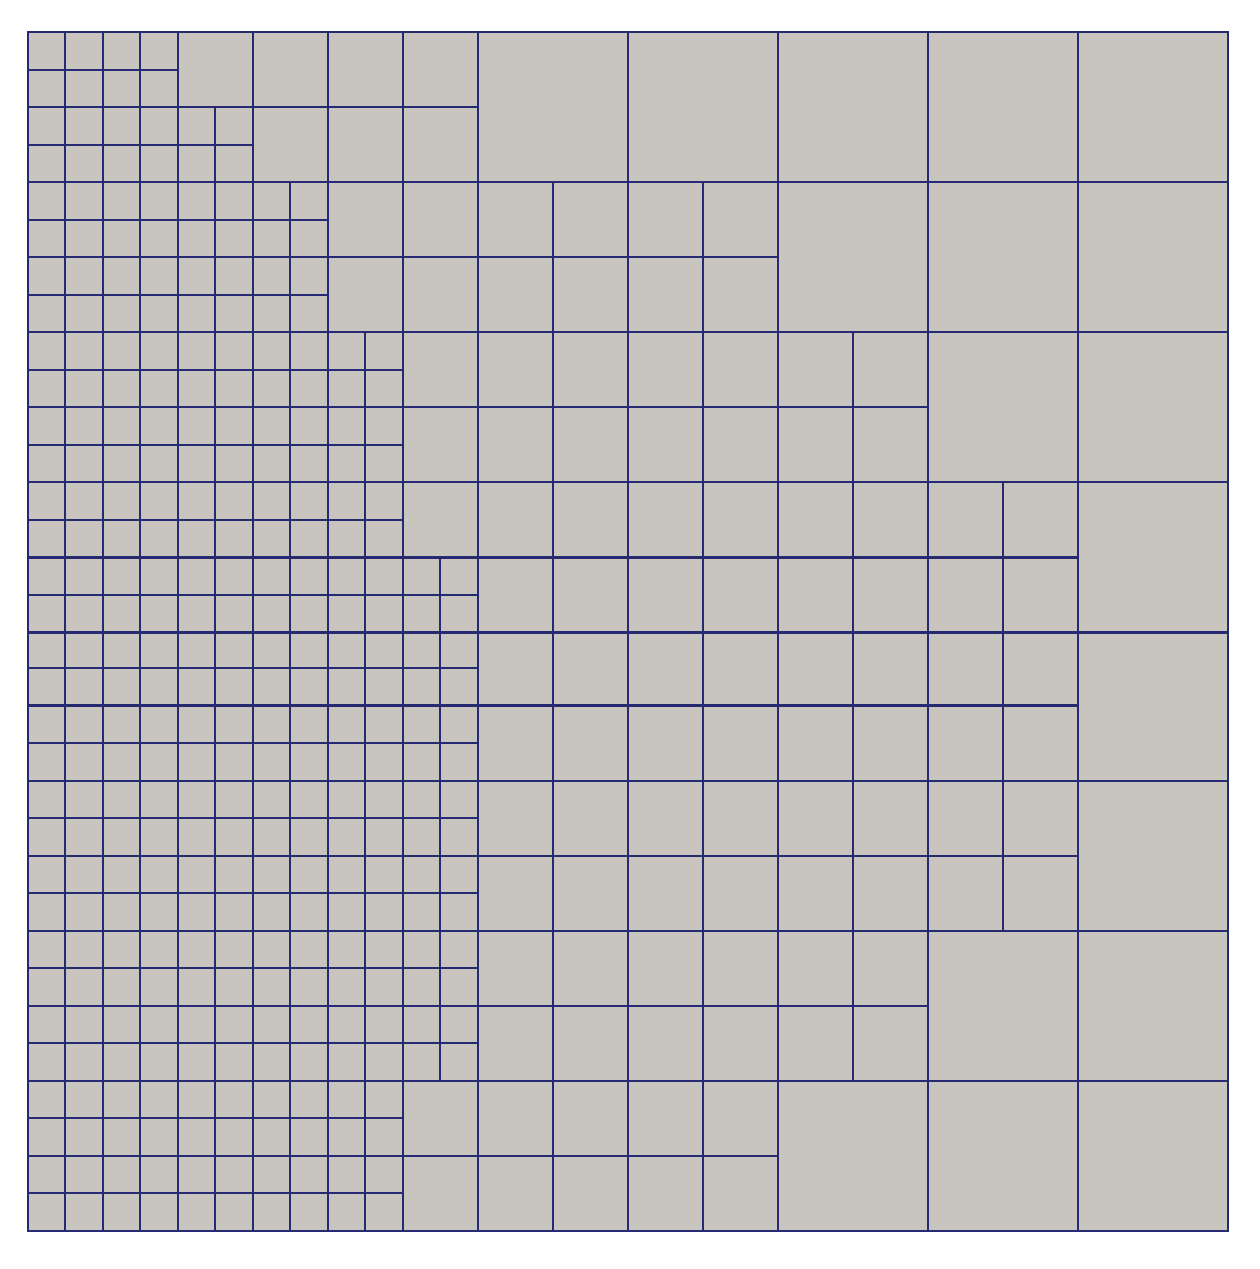
\includegraphics{adaptivity/ex_images/ex_short_cantilever_mesh_992.eps}
        }
        \caption{2nd mesh (992 DOF)}
    \end{subfigure}
    \begin{subfigure}[b]{0.4\linewidth}
        \centering
        \scalebox{0.25}{
            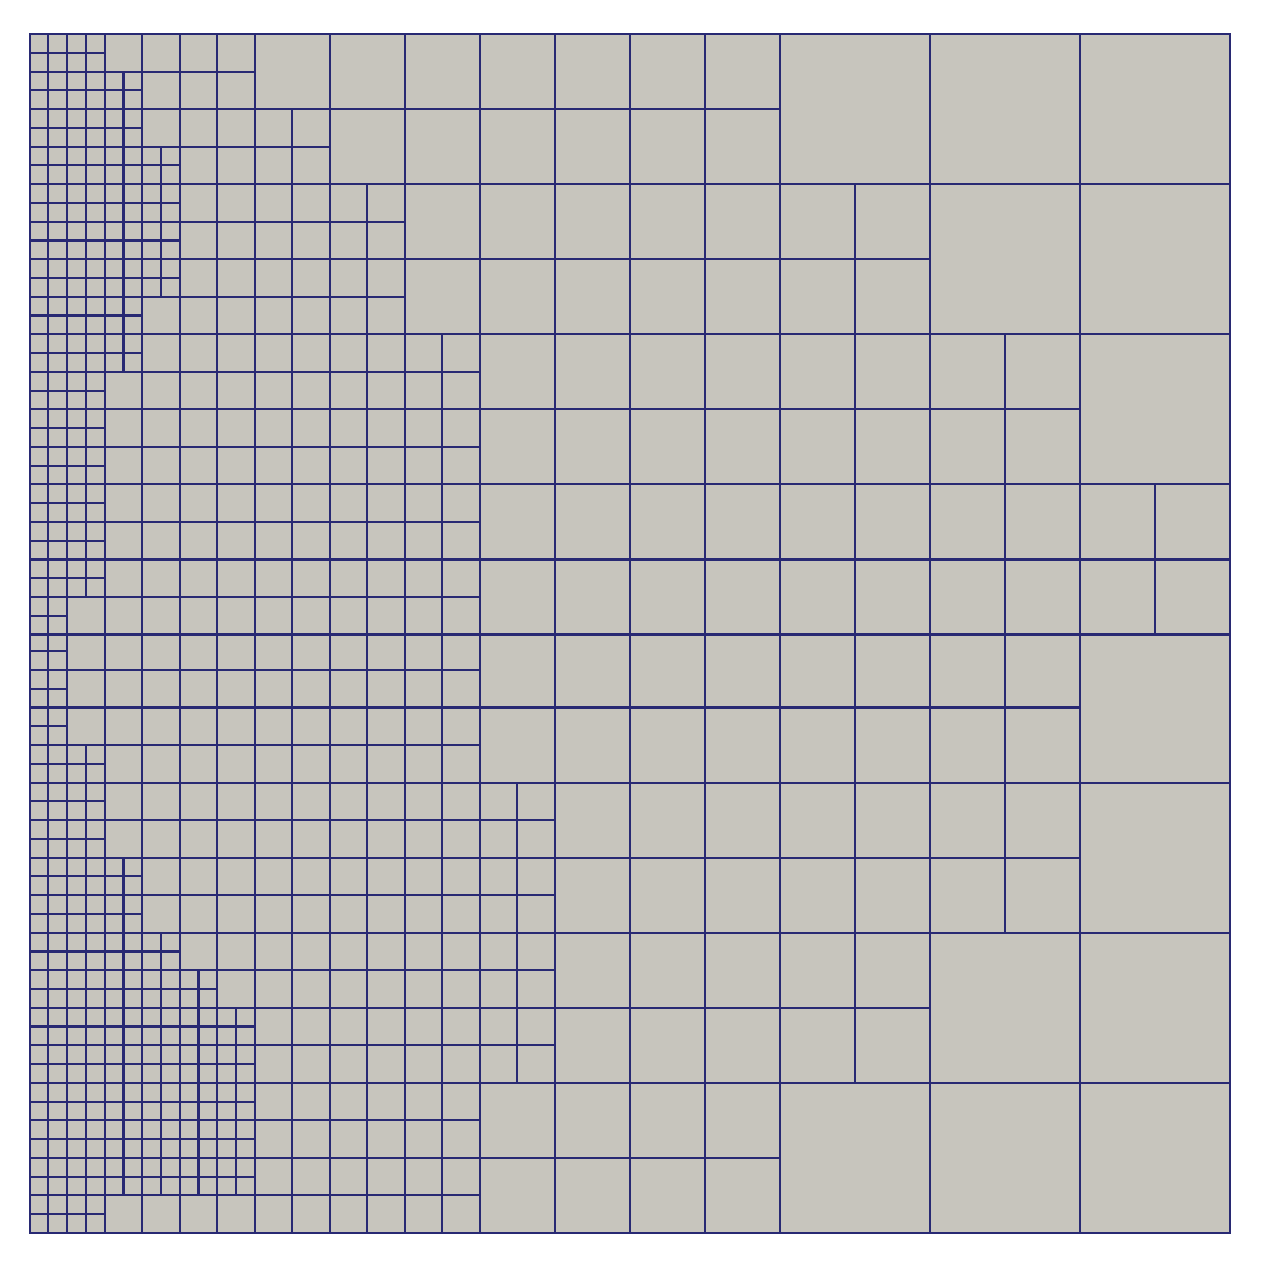
\includegraphics{adaptivity/ex_images/ex_short_cantilever_mesh_1780.eps}
        }
        \caption{3rd refinement (1780 DOF)}
    \end{subfigure}
    \caption{ Short cantilever beam: mesh development (SBFEM)}
    \label{adap_fig:ex_short_cantilever_mesh_develpment}
\end{figure}

\begin{figure}[h!]
    \centering
    \begin{subfigure}[b]{0.48\linewidth}
        \centering
        \scalebox{0.35}{
            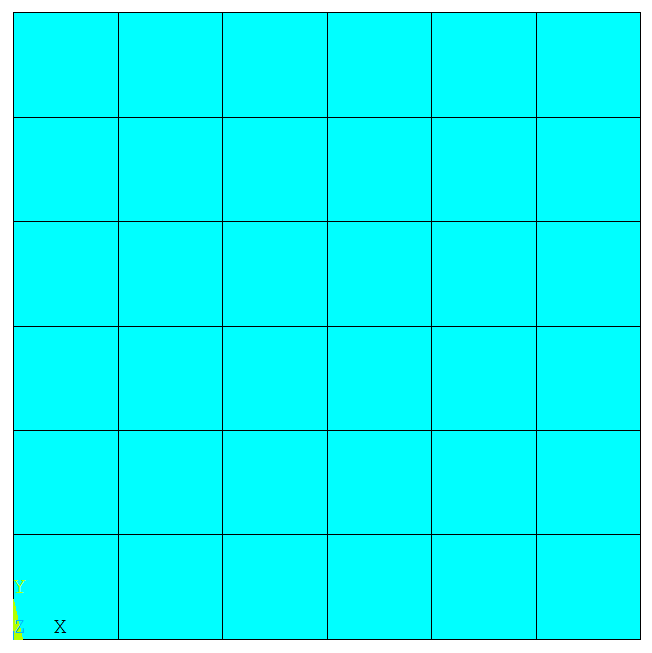
\includegraphics{adaptivity/ex_images/ex_short_cantilever_ansys_2_133.png}
        }
        \caption{Initial mesh, 266 DOFs}
    \end{subfigure}
    \begin{subfigure}[b]{0.48\linewidth}
        \centering
        \scalebox{0.35}{
            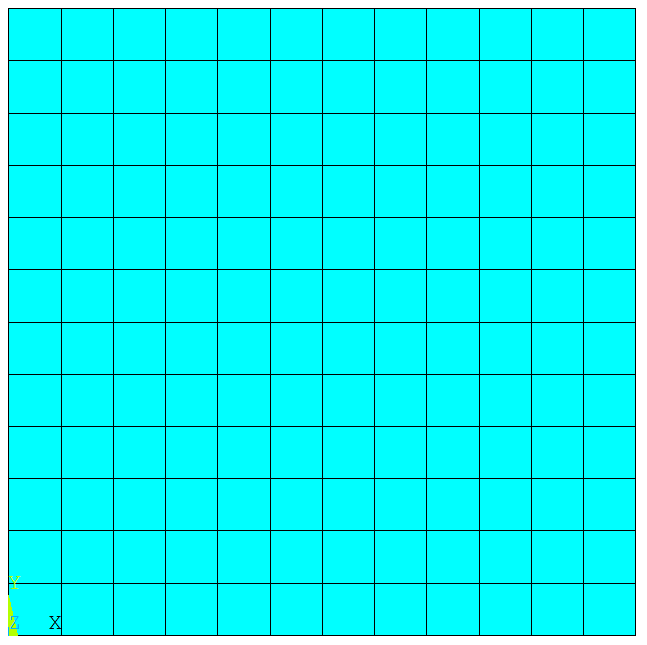
\includegraphics{adaptivity/ex_images/ex_short_cantilever_ansys_2_481.png}
        }
        \caption{1st refinement, 962 DOFs}
    \end{subfigure}
    \begin{subfigure}[b]{0.48\linewidth}
        \centering
        \scalebox{0.35}{
            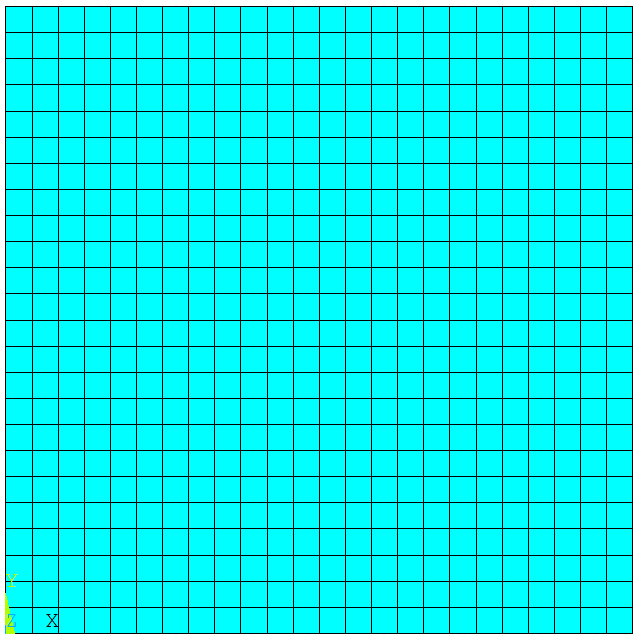
\includegraphics{adaptivity/ex_images/ex_short_cantilever_ansys_2_1825.png}
        }
        \caption{2nd refinement, 3650 DOFs}
    \end{subfigure}
    \begin{subfigure}[b]{0.48\linewidth}
        \centering
        \scalebox{0.35}{
            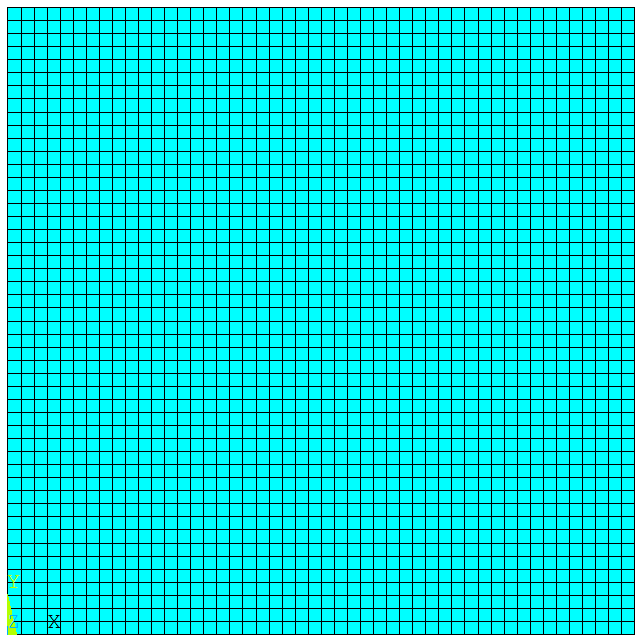
\includegraphics{adaptivity/ex_images/ex_short_cantilever_ansys_2_7105.png}
        }
        \caption{3rd refinement, 14210 DOFs}
    \end{subfigure}
    \caption{Short cantilever beam: mesh development (Ansys)}
    \label{adap_fig:ex_short_cantilever_mesh_develpment_ansys}
\end{figure}

\begin{figure}
    \centering
    \scalebox{0.35}{
        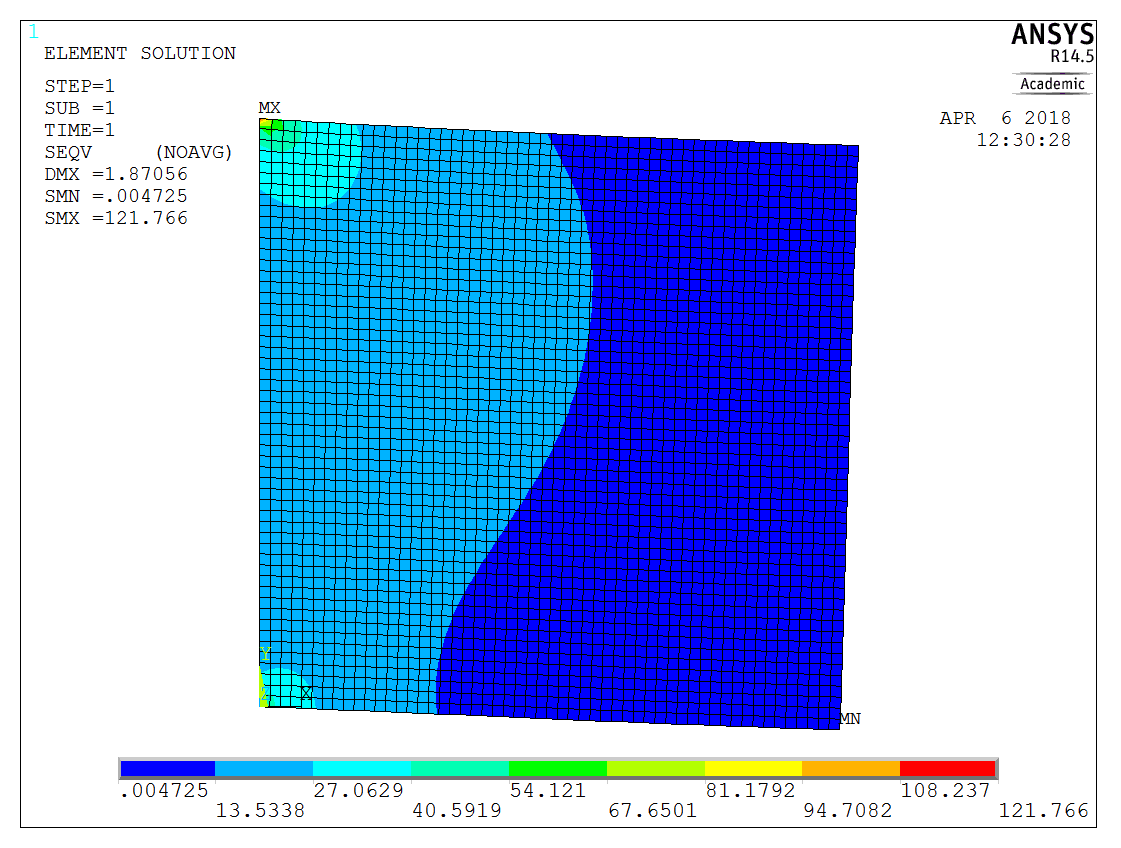
\includegraphics{adaptivity/ex_images/ex_short_cantilever_stress_ansys.png}
    }
    \caption{Von-mises stress contour using 9-node quadrilateral element in ANSYS (17930 DOFs)}
    \label{adap_fig:ex_chole_stress_ansys}
\end{figure}
\pagebreak
% /* cSpell:disable */
%  57205*2 - 11.7733    (ansys 2nd)

% mlp
% 262 - 11.7237
% 940 - 11.7598
% 1408 - 11.7670
% 2176 - 11.7704
% err=abs([11.7237,11.7598,11.7671,11.7704]-11.7733)/11.7733; dof=[262,940,1434,2176]; polyfit(log(dof),log(err),1)

% disperr > 0.005
% 262 - 11.7237
% 664 - 11.7513
% 1112 - 11.7649
% 1316 - 11.7670
% err=abs([11.7237,11.7513,11.7649,11.7670]-11.7733)/11.7733; dof=[262,664,1112,1316]; polyfit(log(dof),log(err),1)

% strerr > 0.01
% 262 - 11.7237
% 860 - 11.7552
% 2792 - 11.7691
% err=abs([11.7237,11.7552,11.7691,]-11.7733)/11.7733; dof=[262,860,2792]; polyfit(log(dof),log(err),1)

% ansys
% 69*2 -> 11.6574
% 241*2 ->  11.7397
% 897*2 -> 11.7646  
% 3457*2 -> 11.7711
% err_a1=abs([11.6574,11.7397,11.7646,11.7711]-11.7733)/11.7733; dof_a1=[69,241,897,3457]*2; polyfit(log(dof_a1),log(err_a1),1)
% /* cSpell:enable */
\subsection{Infinite plate with a circular hole}
\paragraph{}
In this example, an infinite plate with a traction free hole under uniaxial tension $(\sigma = \SI{1}{\newton \per \meter^2} ) $  along y-axis (see Fig.~\ref{adap_fig:ex_chole_geo_bc}) is considered.
\begin{figure}[h!]
    \centering
    \scalebox{1.4}{
        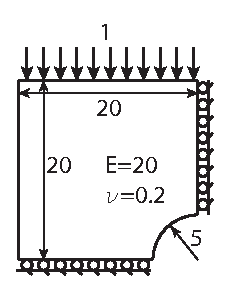
\includegraphics{adaptivity/ex_images/ex_chole_adap_geo_bc.eps}
    }
    \caption{Infinite plate with a circular hole: geometry and boundary conditions}
    \label{adap_fig:ex_chole_geo_bc}
\end{figure}

\paragraph{}
Owing to symmetry, only one quarter of the plate is modeled.
In this example, uniform distributed load are applied on the top and plane stress condition is assumed.
The bottom and right boundary are enforced with a roller boundary condition. $u_y=0$ where $y=0$ and $u_x=0$ where $x=0$.

\paragraph{}
% result analysis
The convergence rate in terms of the total strain energy is shown in Fig.~\ref{adap_fig:ex_chole_conv} and corresponding mesh development are presented in Fig.~\ref{adap_fig:ex_chole_mesh_sbfem} (SBFEM) and Fig.~\ref{adap_fig:ex_chole_mesh_ansys} ( Ansys 4-node quadrilateral element ).
Higher convergence rate compared to the result determined in ANSYS is observed.
\begin{figure}[h!]
    \centering
    \scalebox{0.5}{
        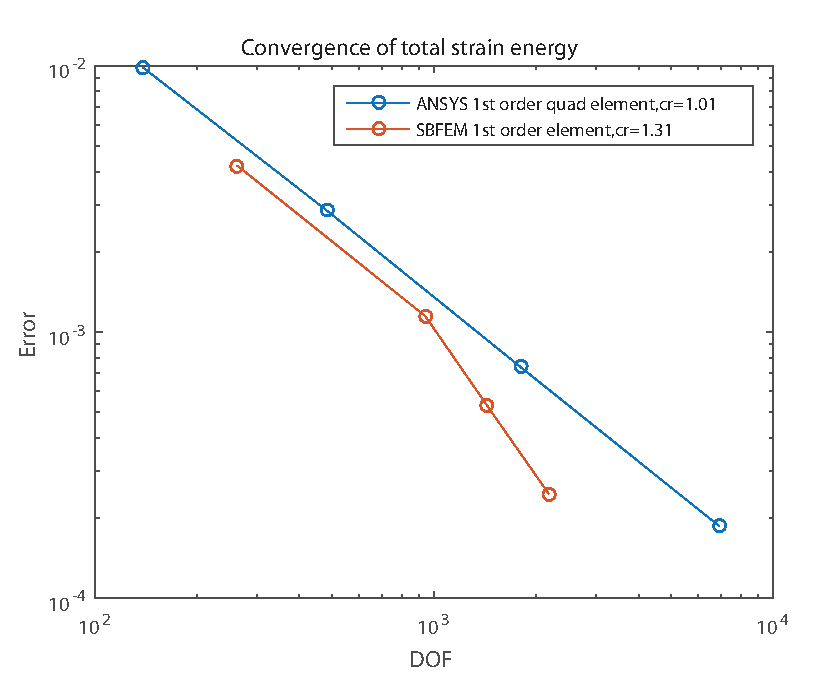
\includegraphics{adaptivity/ex_images/ex_chole_adap_conv.eps}
    }
    \caption{Infinite plate with a circular hole: Convergence study}
    \label{adap_fig:ex_chole_conv}
\end{figure}

\begin{figure}[h!]
    \centering
    \begin{subfigure}[b]{0.4\linewidth}
        \centering
        \scalebox{0.3}{
            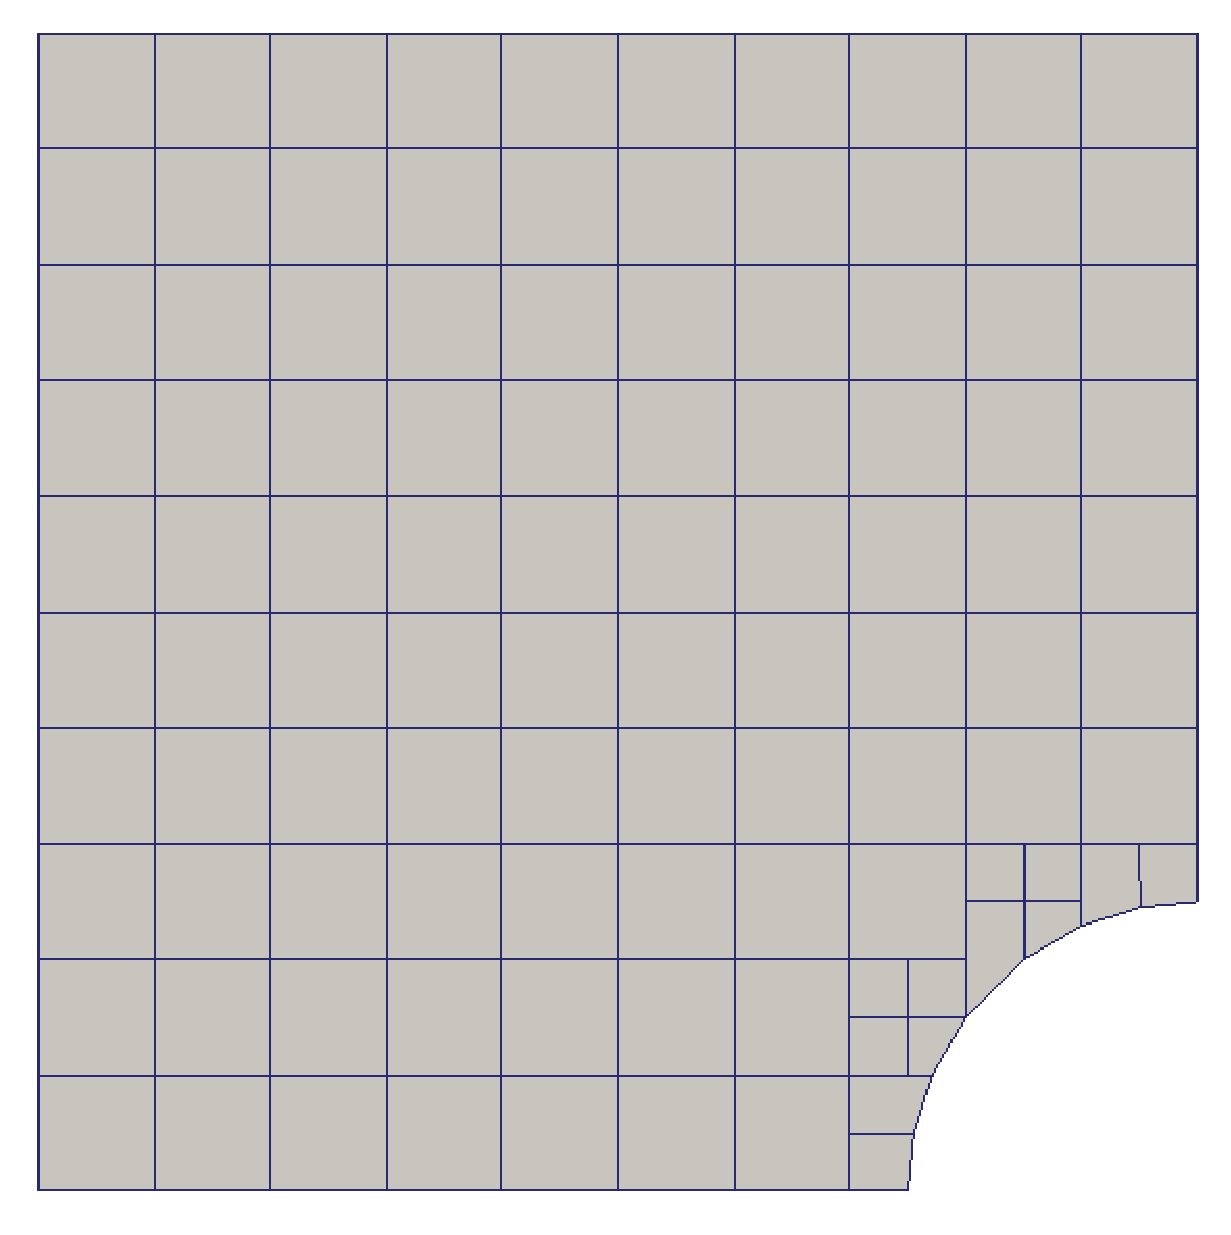
\includegraphics{adaptivity/ex_images/ex_chole_adap_131.eps}
        }
        \caption{Initial mesh, 131 DOFs}
    \end{subfigure}
    \begin{subfigure}[b]{0.4\linewidth}
        \centering
        \scalebox{0.3}{
            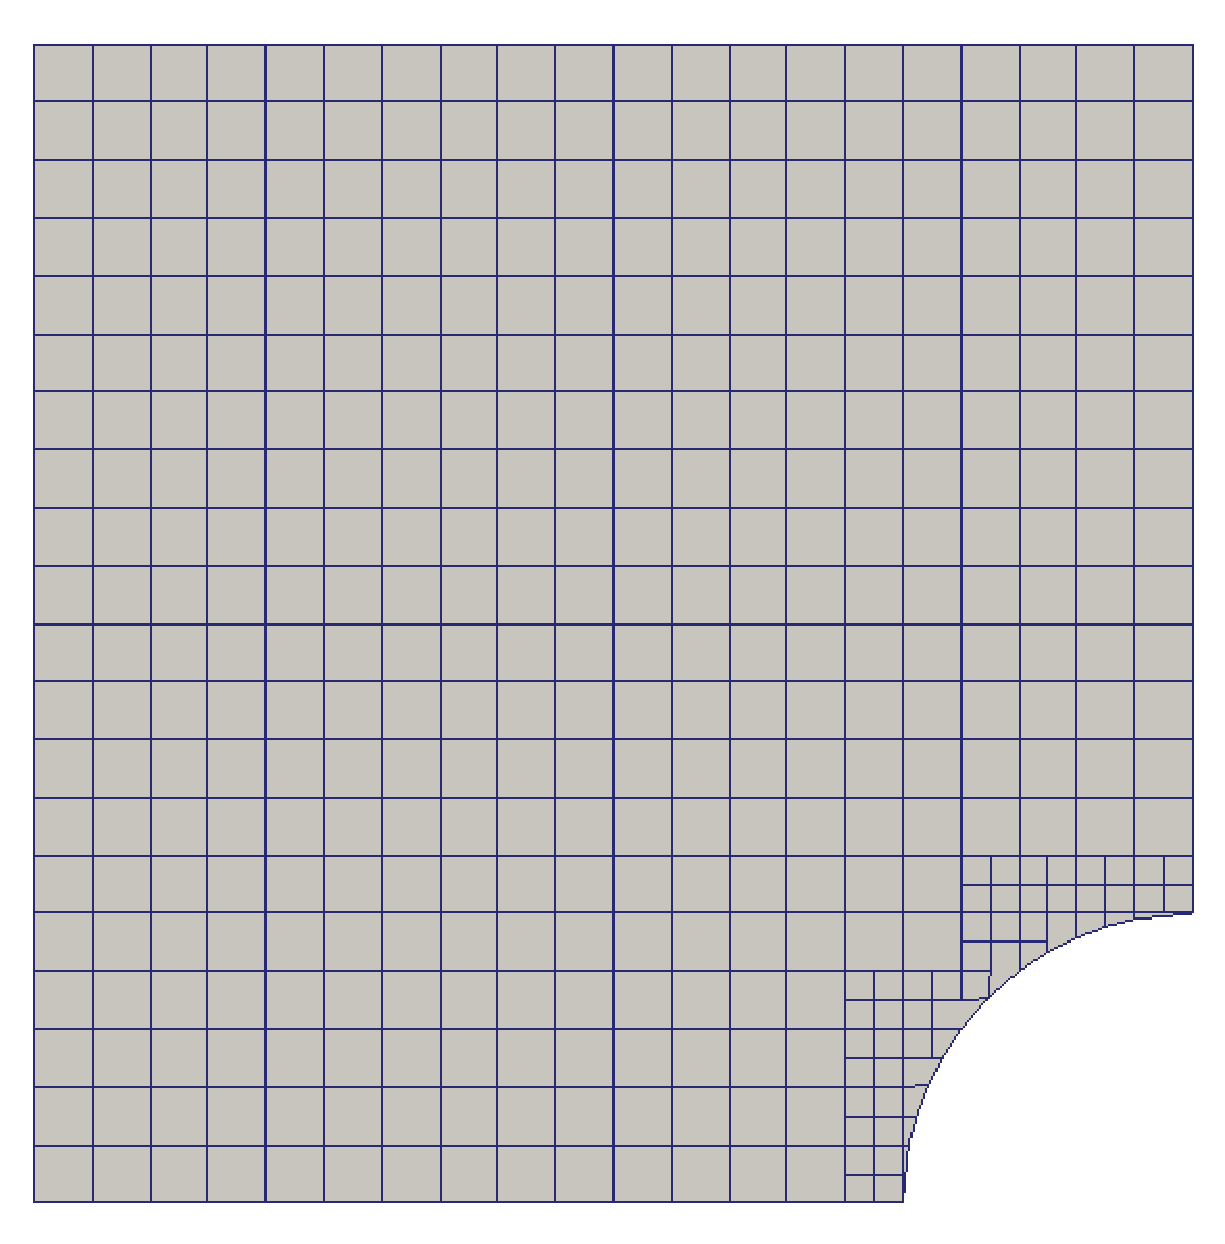
\includegraphics{adaptivity/ex_images/ex_chole_adap_472.eps}
        }
        \caption{1st refinement, 472 DOFs}
    \end{subfigure}
    \begin{subfigure}[b]{0.4\linewidth}
        \centering
        \scalebox{0.3}{
            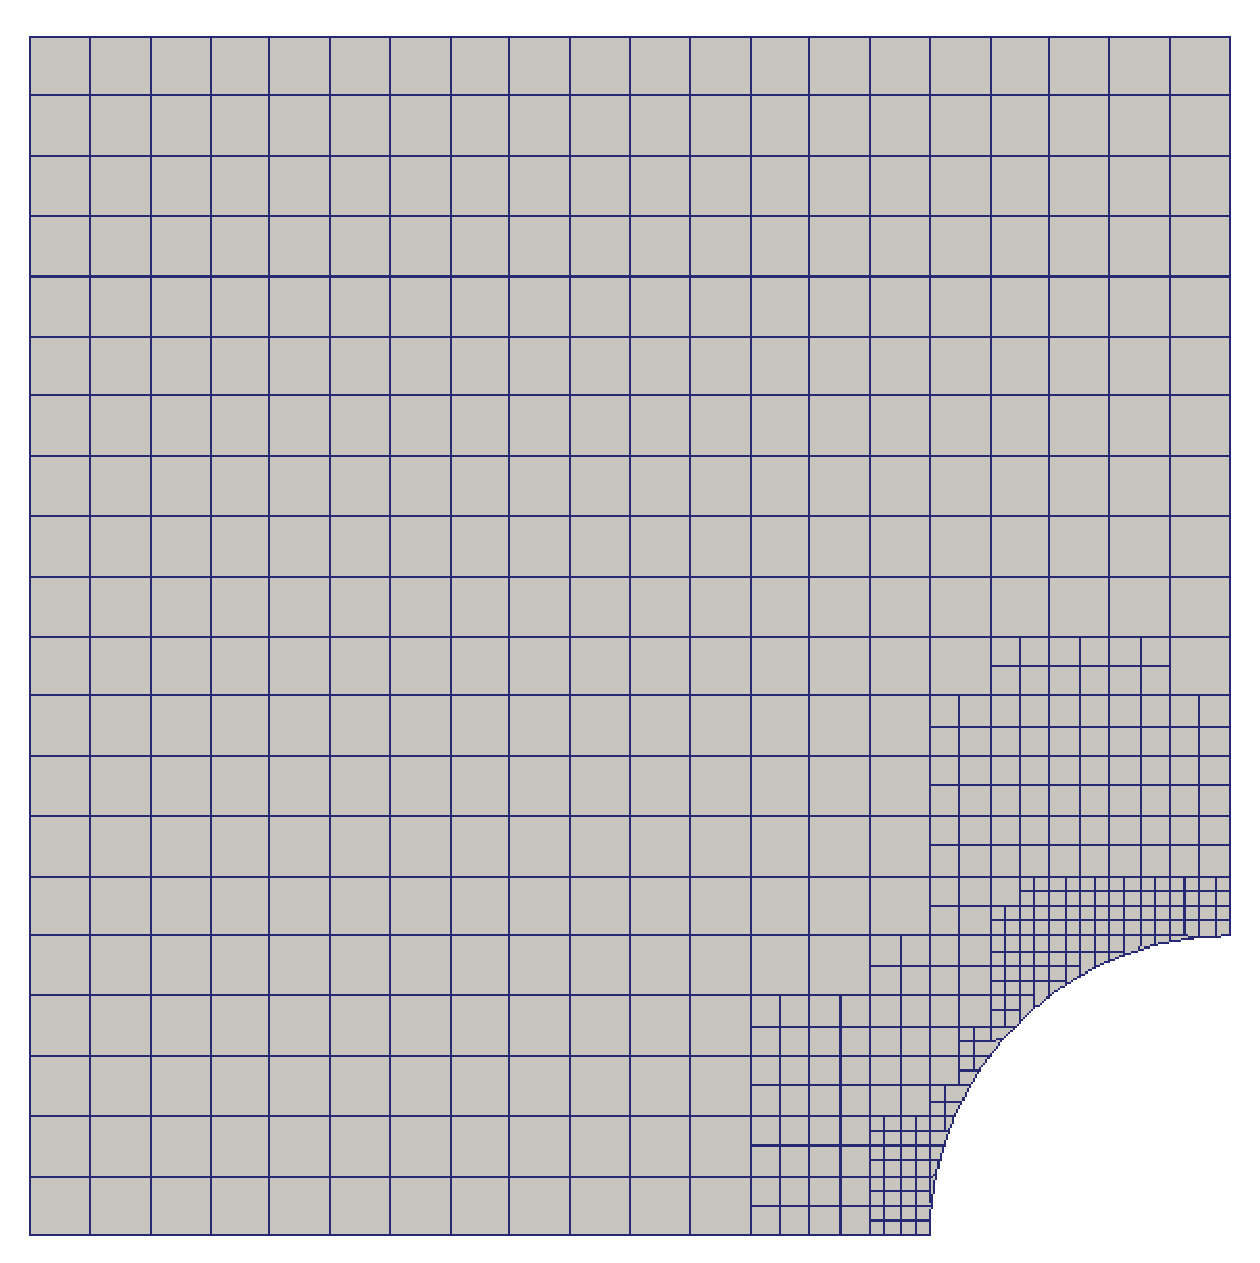
\includegraphics{adaptivity/ex_images/ex_chole_adap_700.eps}
        }
        \caption{2nd refinement, 700 DOFs}
    \end{subfigure}
    \begin{subfigure}[b]{0.4\linewidth}
        \centering
        \scalebox{0.3}{
            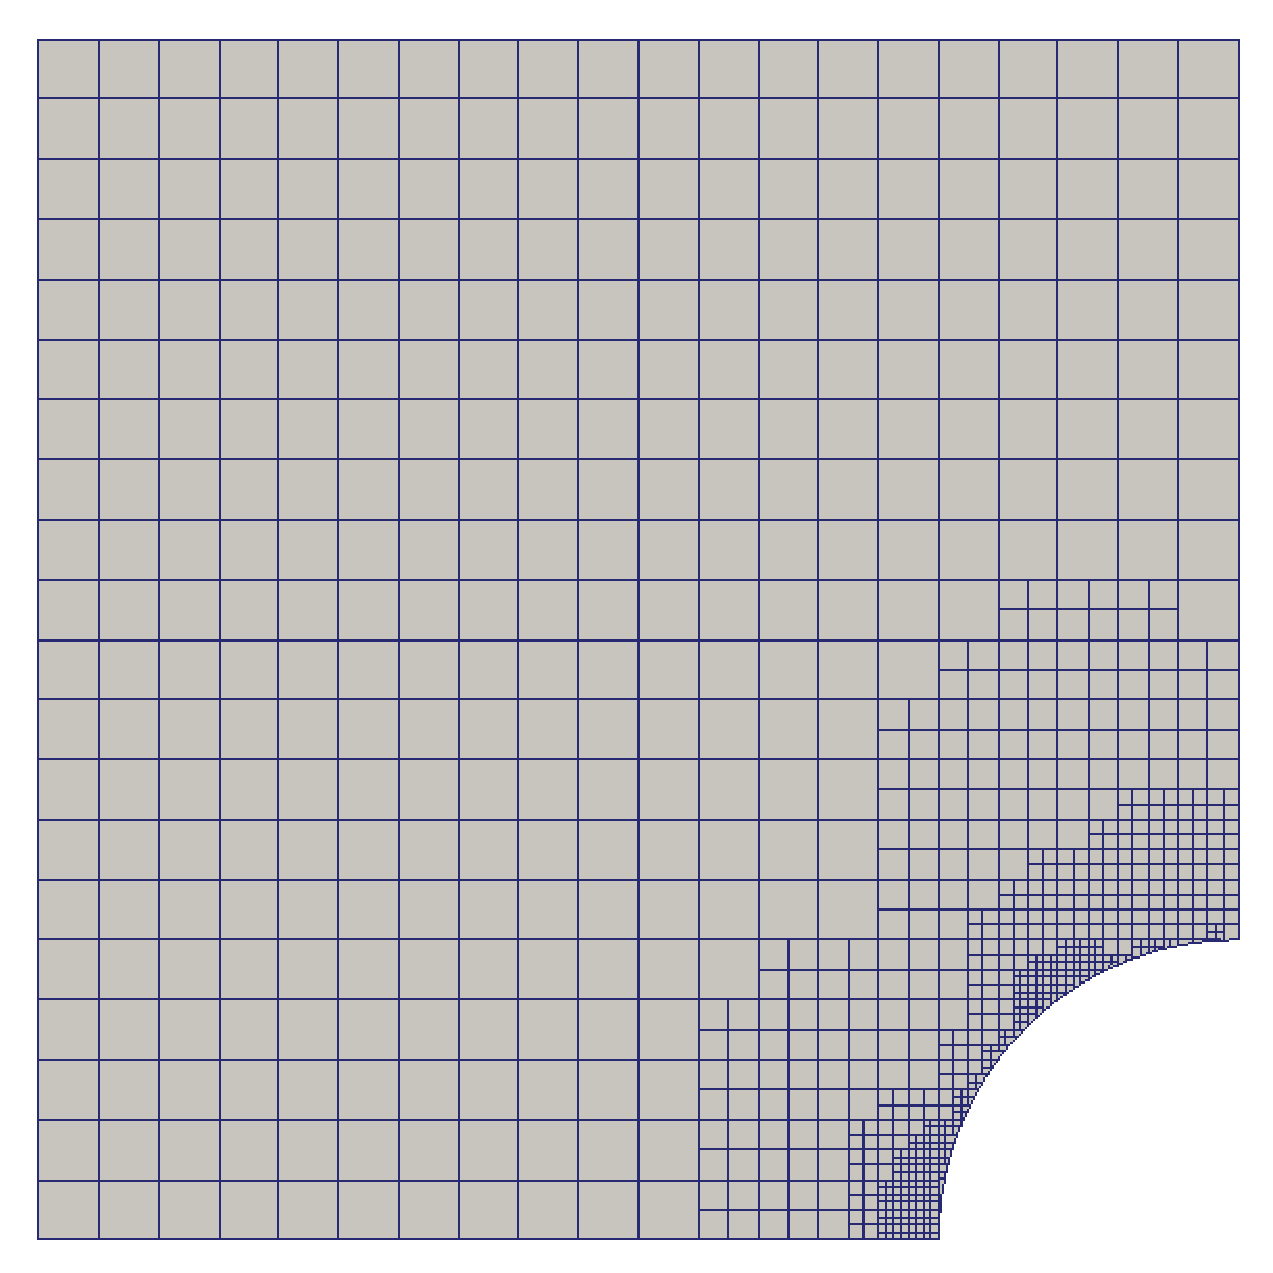
\includegraphics{adaptivity/ex_images/ex_chole_adap_1075.eps}
        }
        \caption{3rd refinement, 1075 DOFs}
    \end{subfigure}
    \caption{Infinite plate with a circular hole: Mesh development (SBFEM)}
    \label{adap_fig:ex_chole_mesh_sbfem}
\end{figure}

\begin{figure}[h!]
    \centering
    \begin{subfigure}[b]{0.48\linewidth}
        \centering
        \scalebox{0.4}{
            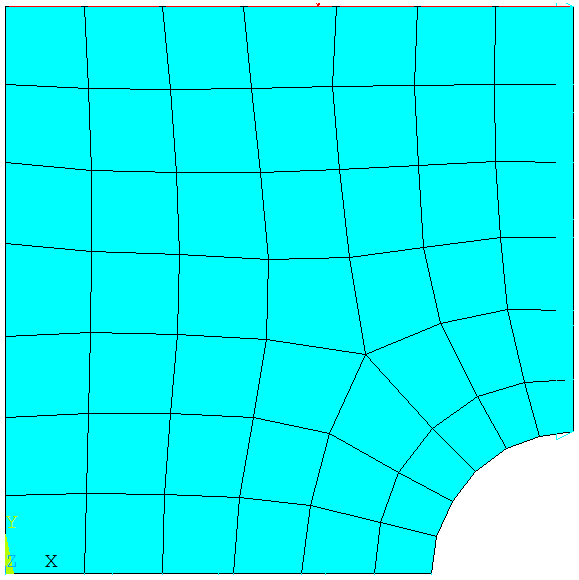
\includegraphics{adaptivity/ex_images/ex_chole_ansys_1_69.png}
        }
        \caption{Initial mesh, 138 DOFs}
    \end{subfigure}
    \begin{subfigure}[b]{0.48\linewidth}
        \centering
        \scalebox{0.4}{
            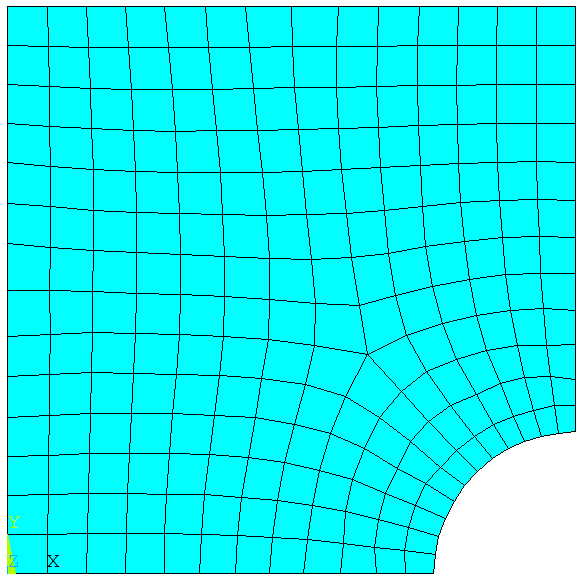
\includegraphics{adaptivity/ex_images/ex_chole_ansys_1_241.png}
        }
        \caption{1st refinement, 482 DOFs}
    \end{subfigure}
    \begin{subfigure}[b]{0.48\linewidth}
        \centering
        \scalebox{0.4}{
            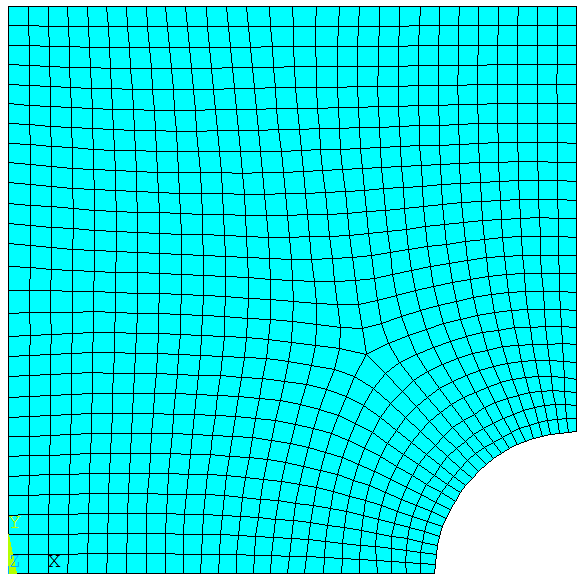
\includegraphics{adaptivity/ex_images/ex_chole_ansys_1_897.png}
        }
        \caption{2nd refinement, 1794 DOFs}
    \end{subfigure}
    \begin{subfigure}[b]{0.48\linewidth}
        \centering
        \scalebox{0.4}{
            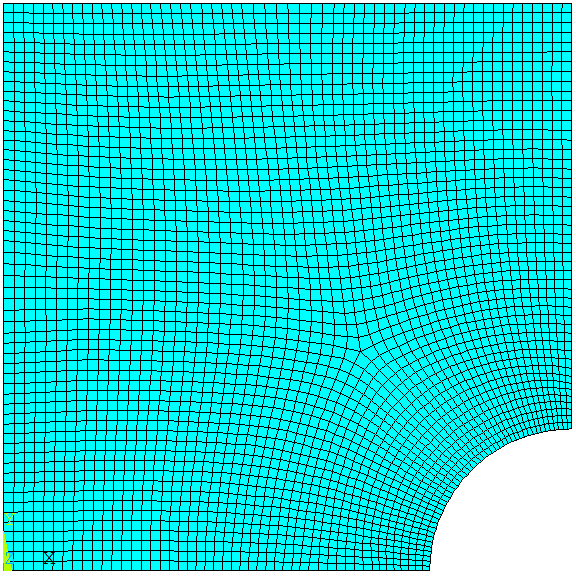
\includegraphics{adaptivity/ex_images/ex_chole_ansys_1_3457.png}
        }
        \caption{3rd refinement, 6914 DOFs}
    \end{subfigure}
    \caption{Infinite plate with a circular hole: Mesh development (Ansys)}
    \label{adap_fig:ex_chole_mesh_ansys}
\end{figure}

\begin{figure}
    \centering
    \scalebox{0.5}{
        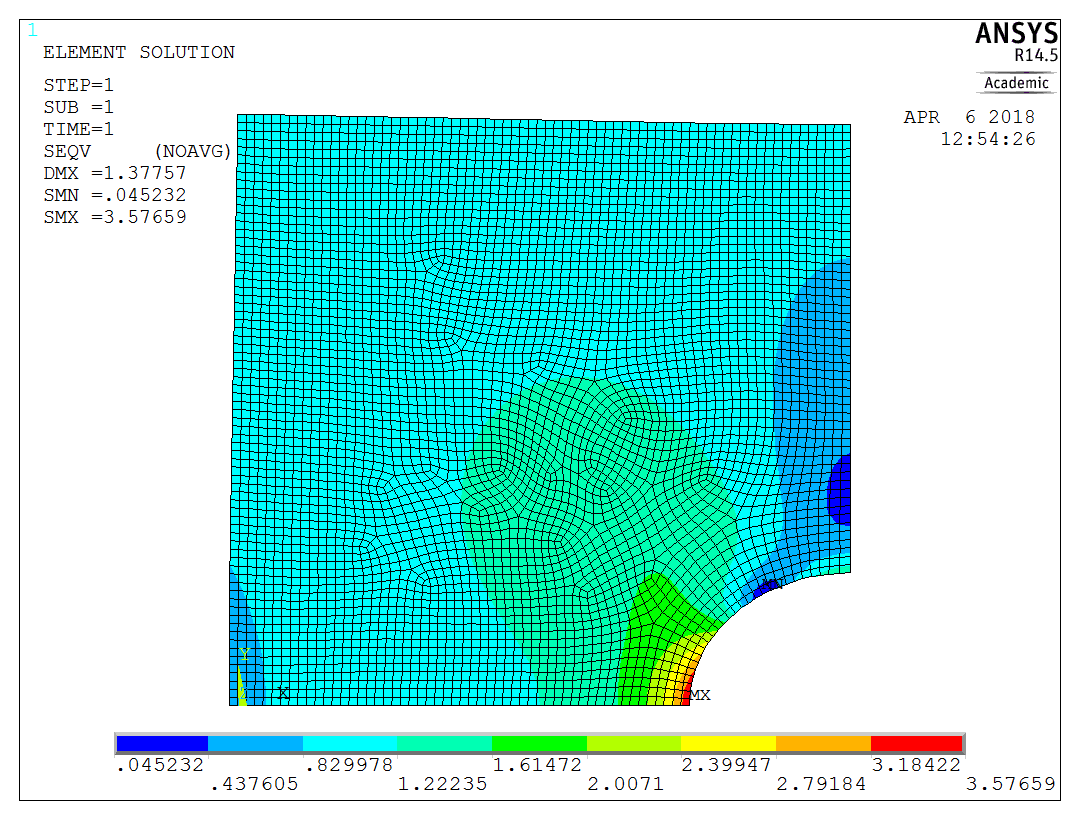
\includegraphics{adaptivity/ex_images/ex_chole_stress_ansys.png}
    }
    \caption{Von-mises stress contour using 9-node quadrilateral element in ANSYS (28450 DOFs)}
    \label{adap_fig:ex_chole_stress_ansys}
\end{figure}

\paragraph{}
In this example, a plane strain bracket with a downward uniform distributed load on the top is considered (see fig.~\ref{adp_fig:ex_bracket_geo_bc}).
The material properties are: Young’s modulus $E = 2\times 10^5 N/m^2$ and Poisson’s ratio $\nu = 0.3$.
    \begin{figure}[H]
        \centering
        \begin{subfigure}[b]{1\linewidth}
            \centering
            \scalebox{1.2}{
                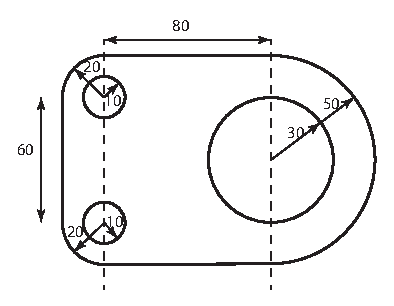
\includegraphics{quadtree/ex_images/ex_bracket_geo.eps}
            }
        \end{subfigure}
        \begin{subfigure}[b]{1\linewidth}
            \centering
            \scalebox{1.3}{
                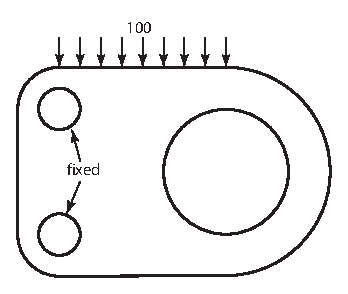
\includegraphics{quadtree/ex_images/ex_bracket_load.eps}
            }
        \end{subfigure}
        \caption{ Plane strain bracket: geometry and boundary conditions}
        \label{adp_fig:ex_bracket_geo_bc}
    \end{figure}

\paragraph{}
A total strain energy of $282.927$ is determined by ANSYS with the mesh shown in fig.~\ref{qdt_fig:ex_bracket_ansys_mesh}

% /* cSpell:disable */
% -1 - 282.927
% 382*2  - 274.5638 (32-4/8-3)
% 950*2  - 280.1255 (64-4/8-3)
% 2110*2 - 281.0799 (128-4/15-4)
% 4414*2 - 282.0363 (256-4/15-4)


% mlp
% 530 - 279.8076
% 1554 - 282.0745
% 4208 - 282.5681
% err = abs([279.8076 ,282.0745,282.5681]-282.927)/282.927; dof = [530,1554,4208]; polyfit(log(dof),log(err),1)

% uniform
% 530 - 279.8076
% 1810 - 282.3186
% 6464 - 282.674
% err_un = abs([279.8076 ,282.3186 ,282.674]-282.927)/282.927; dof_un = [530,1810,6464]; polyfit(log(dof_un),log(err_un),1)

% ansys-2nd
% 406*2 -  282.412
% 1144*2 - 282.895
% 4270*2 - 282.923

% 16462*2 -  282.926
% err_a2 = abs([282.412,282.895,282.923]-282.927)/282.927; dof_a2 = [406,1144,4270]*2; polyfit(log(dof_a2),log(err_a2),1)

% ansys-1st
% 185*2 - 275.635    
% 650*2 -  280.006   
% 1227*2 -  281.502 
% 2405*2 - 282.136
% err_a1 = abs([275.635,280.006  ,281.502 ,282.136]-282.927)/282.927; dof_a1 = [185,650,1227,2405]*2; polyfit(log(dof_a1),log(err_a1),1)

% disp > 0.01
% 530 - 279.8076
% 1348 - 281.4530
% 2768 - 282
% 5438 - 282.2
% err_d = abs([279.8076, 281.4530  ,282 ,282.2]-282.927)/282.927; dof_d = [530,1348,2768,5438]; polyfit(log(dof_d),log(err_d),1)

% str > 0.1
% 530 - 279.8076
% 1514 - 281.8970
% 4336 - 282.1295

% err_s = abs([279.8076, 281.8970  ,282.1295 ]-282.927)/282.927; dof_s = [530,1514,4336]; polyfit(log(dof_s),log(err_s),1)


% /* cSpell:enable */
\paragraph{}
% result analysis
The convergence rate in terms of the total strain energy is shown in Fig.~\ref{adap_fig:ex_bracket_conv} and corresponding mesh development are presented in Fig.~\ref{adap_fig:ex_bracket_mesh_sbfem} (SBFEM) and Fig.~\ref{adap_fig:ex_bracket_mesh_ansys} ( Ansys 4-node quadrilateral element ).
Higher convergence rate compared to the result determined in ANSYS is observed.

\begin{figure}[h!]
    \centering
    \scalebox{0.5}{
        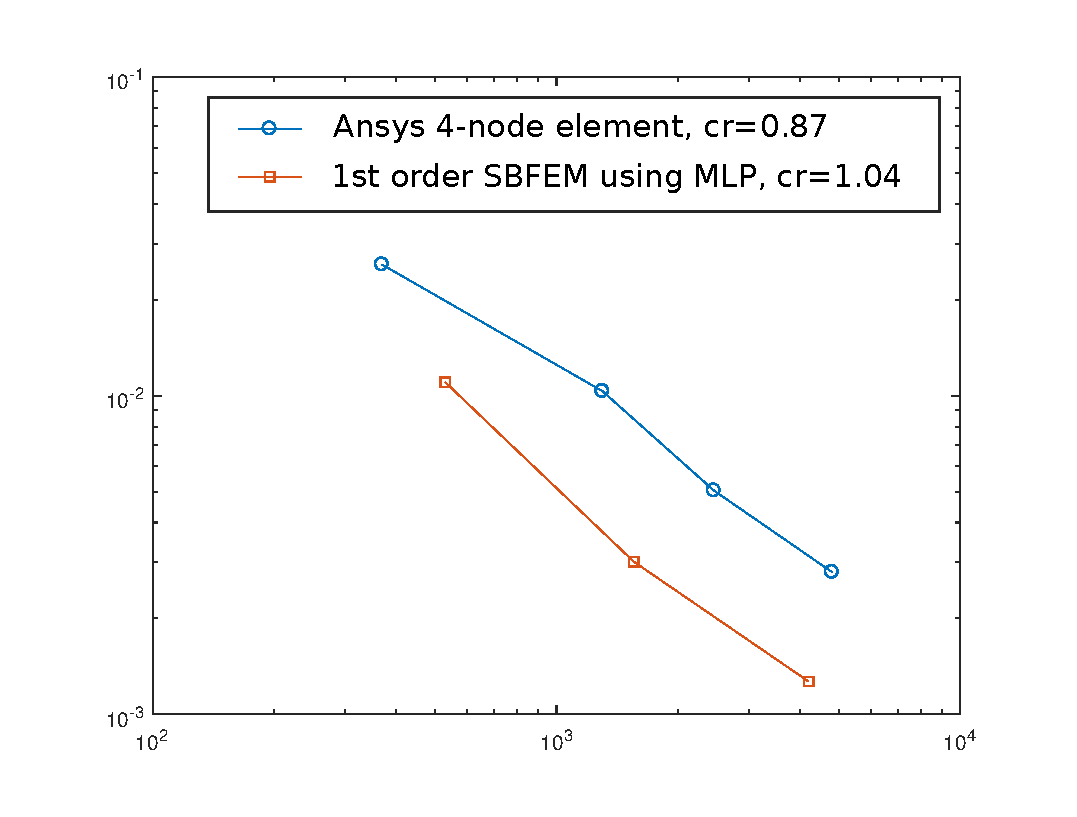
\includegraphics{adaptivity/ex_images/ex_adap_bracket_conv.eps}
    }
    \caption{Plane strain bracket: Convergence study}
    \label{adap_fig:ex_bracket_conv}
\end{figure}

\begin{figure}[h!]
    \centering
    \begin{subfigure}[b]{0.4\linewidth}
        \centering
        \scalebox{0.6}{
            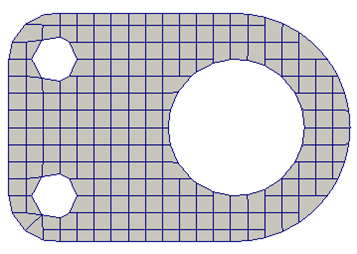
\includegraphics{adaptivity/ex_images/ex_adap_bracket_530.png}
        }
        \caption{Initial mesh, 530 DOFs}
    \end{subfigure}
    \begin{subfigure}[b]{0.4\linewidth}
        \centering
        \scalebox{0.6}{
            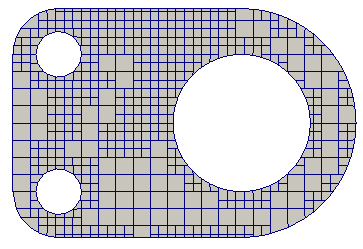
\includegraphics{adaptivity/ex_images/ex_adap_bracket_1554.png}
        }
        \caption{1st refinement, 1554 DOFs}
    \end{subfigure}
    \begin{subfigure}[b]{0.4\linewidth}
        \centering
        \scalebox{0.6}{
            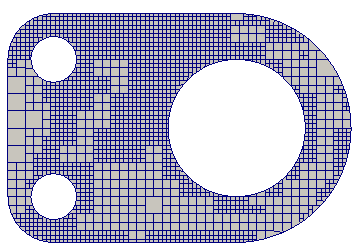
\includegraphics{adaptivity/ex_images/ex_adap_bracket_4208.png}
        }
        \caption{2nd refinement, 4208 DOFs}
    \end{subfigure}
    \caption{Plane strain bracket: Mesh development (SBFEM)}
    \label{adap_fig:ex_bracket_mesh_sbfem}
\end{figure}


\begin{figure}[h!]
    \centering
    \begin{subfigure}[b]{0.48\linewidth}
        \centering
        \scalebox{0.4}{
            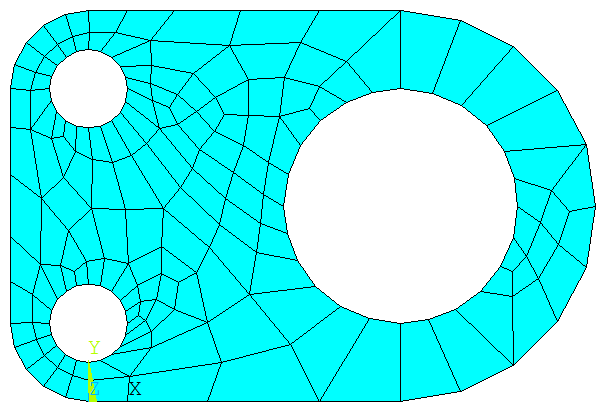
\includegraphics{adaptivity/ex_images/ex_adp_bracket_ansys_185.png}
        }
        \caption{Initial mesh, 138 DOFs}
    \end{subfigure}
    \begin{subfigure}[b]{0.48\linewidth}
        \centering
        \scalebox{0.4}{
            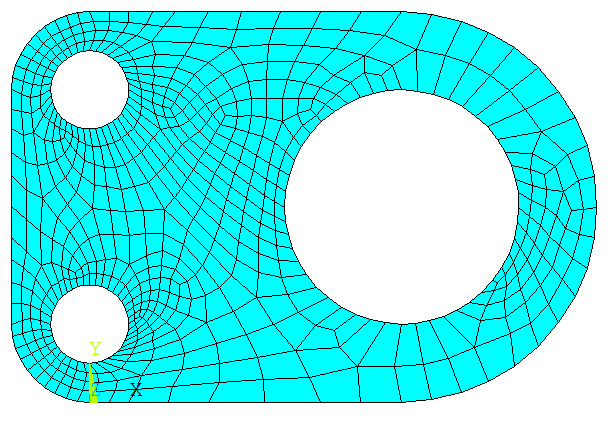
\includegraphics{adaptivity/ex_images/ex_adp_bracket_ansys_650.png}
        }
        \caption{1st refinement, 482 DOFs}
    \end{subfigure}
    \begin{subfigure}[b]{0.48\linewidth}
        \centering
        \scalebox{0.4}{
            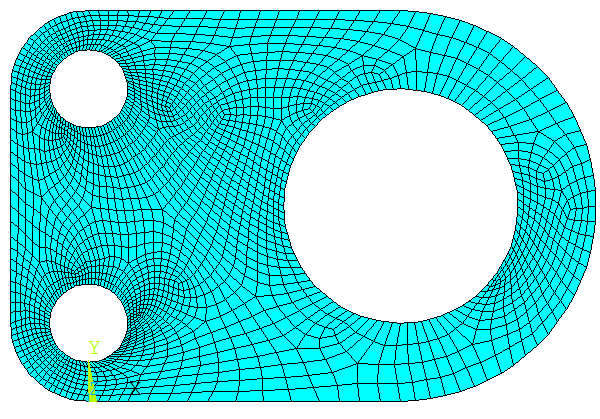
\includegraphics{adaptivity/ex_images/ex_adp_bracket_ansys_1227.png}
        }
        \caption{2nd refinement, 1794 DOFs}
    \end{subfigure}
    \begin{subfigure}[b]{0.48\linewidth}
        \centering
        \scalebox{0.4}{
            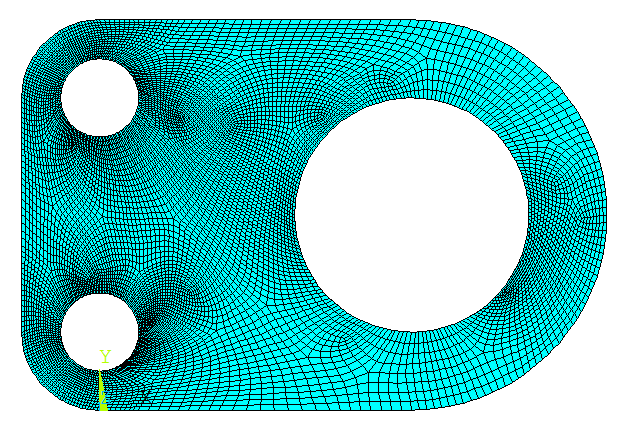
\includegraphics{adaptivity/ex_images/ex_adp_bracket_ansys_2405.png}
        }
        \caption{3rd refinement, 6914 DOFs}
    \end{subfigure}
    \caption{Plane strain bracket: Mesh development (Ansys)}
    \label{adap_fig:ex_bracket_mesh_ansys}
\end{figure}

\section{Conclusions}
\paragraph{}
In this chapter, the machine learning algorithm is adopted to develop an extensible and flexible error indicator.
Any other error estimators can be added to the existing framework and their effects can be detected based on the performance indicators in machine learning.
A MLP trained error estimator that concludes expressions related to the eigenvalues of the SBFEM formulation and some key geometric properties of the scaled boundary finite element give a higher convergence rate compared to the uniform refinement.
In order to improve the learning effectiveness of the MLP, regularization methods including bagging and dropout are utilized.
Due to the lack of the eigenvalue error indicator in the first order triangular element, method that eliminates these situation is developed.
A matrix representation of the NURBS curves is presented to achieve a higher efficiency and stability in calculating the intersections between edge\hl{s} of the element and the NURBS curve.
Stress analysis is conducted on 2D linear elasticity problems.